%&preformat-synopsis
\RequirePackage[l2tabu,orthodox]{nag} % Раскомментировав, можно в логе получать рекомендации относительно правильного использования пакетов и предупреждения об устаревших и нерекомендуемых пакетах
\PassOptionsToPackage{bookmarks=false}{hyperref}
\documentclass[a5paper,10pt,twoside,openany,article]{memoir} %,draft

%%%%%%%%%%%%%%%%%%%%%%%%%%%%%%%%%%%%%%%%%%%%%%%%%%%%%%
%%%% Файл упрощённых настроек шаблона диссертации %%%%
%%%%%%%%%%%%%%%%%%%%%%%%%%%%%%%%%%%%%%%%%%%%%%%%%%%%%%

%%% Инициализирование переменных, не трогать!  %%%
\newcounter{tabcap}
\newcounter{tablaba}
\newcounter{tabtita}
\newcounter{showperssign}
\newcounter{showsecrsign}
\newcounter{showopplead}
\newcounter{usefootcite}
%%%%%%%%%%%%%%%%%%%%%%%%%%%%%%%%%%%%%%%%%%%%%%%%%%

%%% Область упрощённого управления оформлением %%%

%% Управление зазором между подрисуночной подписью и основным текстом
\setlength{\belowcaptionskip}{10pt plus 20pt minus 2pt}


%% Подпись таблиц
\setcounter{tabcap}{0}              % 0 --- по ГОСТ, номер таблицы и название разделены тире, выровнены по левому краю, при необходимости на нескольких строках; 1 --- подпись таблицы не по ГОСТ, на двух и более строках, дальнейшие настройки: 
%Выравнивание первой строки, с подписью и номером
\setcounter{tablaba}{2}             % 0 --- по левому краю; 1 --- по центру; 2 --- по правому краю
%Выравнивание строк с самим названием таблицы
\setcounter{tabtita}{1}             % 0 --- по левому краю; 1 --- по центру; 2 --- по правому краю
%Разделитель записи «Таблица #» и названия таблицы
\newcommand{\tablabelsep}{ }

%% Подпись рисунков
%Разделитель записи «Рисунок #» и названия рисунка
\newcommand{\figlabelsep}{~\cyrdash\ } % (ГОСТ 2.105, 4.3.1) % "--- здесь не работает

%Демонстрация подписи диссертанта на автореферате
\setcounter{showperssign}{1}        % 0 --- не показывать; 1 --- показывать
%Демонстрация подписи учёного секретаря на автореферате
\setcounter{showsecrsign}{1}        % 0 --- не показывать; 1 --- показывать
%Демонстрация информации об оппонентах и ведущей организации на автореферате
\setcounter{showopplead}{1}         % 0 --- не показывать; 1 --- показывать

%%% Цвета гиперссылок %%%
% Latex color definitions: http://latexcolor.com/
%\definecolor{linkcolor}{rgb}{0.9,0,0}
%\definecolor{citecolor}{rgb}{0,0.6,0}
%\definecolor{urlcolor}{rgb}{0,0,1}
\definecolor{linkcolor}{rgb}{0,0,0} %black
\definecolor{citecolor}{rgb}{0,0,0} %black
\definecolor{urlcolor}{rgb}{0,0,0} %black

%%% Библиография
\setcounter{usefootcite}{0}         % 0 --- два списка литературы, 1 --- список публикаций автора + цитирование других работ в сносках
          % общие настройки шаблона
\input{common/packages}       % Пакеты общие для диссертации и автореферата
\synopsistrue                 % Этот документ --- автореферат
\input{Synopsis/synpackages}  % Пакеты для автореферата
\input{Synopsis/userpackages} % Пакеты для специфических пользовательских задач

\input{common/newnames}       % Новые переменные, которые могут использоваться во всём проекте
%%%%%%%%%%%%%%%%%%%%%%%%%%%%%%%%%%%%%%%%%%%%%%%%%%%%%%
%%%% Файл упрощённых настроек шаблона диссертации %%%%
%%%%%%%%%%%%%%%%%%%%%%%%%%%%%%%%%%%%%%%%%%%%%%%%%%%%%%

%%% Инициализирование переменных, не трогать!  %%%
\newcounter{tabcap}
\newcounter{tablaba}
\newcounter{tabtita}
\newcounter{showperssign}
\newcounter{showsecrsign}
\newcounter{showopplead}
\newcounter{usefootcite}
%%%%%%%%%%%%%%%%%%%%%%%%%%%%%%%%%%%%%%%%%%%%%%%%%%

%%% Область упрощённого управления оформлением %%%

%% Управление зазором между подрисуночной подписью и основным текстом
\setlength{\belowcaptionskip}{10pt plus 20pt minus 2pt}


%% Подпись таблиц
\setcounter{tabcap}{0}              % 0 --- по ГОСТ, номер таблицы и название разделены тире, выровнены по левому краю, при необходимости на нескольких строках; 1 --- подпись таблицы не по ГОСТ, на двух и более строках, дальнейшие настройки: 
%Выравнивание первой строки, с подписью и номером
\setcounter{tablaba}{2}             % 0 --- по левому краю; 1 --- по центру; 2 --- по правому краю
%Выравнивание строк с самим названием таблицы
\setcounter{tabtita}{1}             % 0 --- по левому краю; 1 --- по центру; 2 --- по правому краю
%Разделитель записи «Таблица #» и названия таблицы
\newcommand{\tablabelsep}{ }

%% Подпись рисунков
%Разделитель записи «Рисунок #» и названия рисунка
\newcommand{\figlabelsep}{~\cyrdash\ } % (ГОСТ 2.105, 4.3.1) % "--- здесь не работает

%Демонстрация подписи диссертанта на автореферате
\setcounter{showperssign}{1}        % 0 --- не показывать; 1 --- показывать
%Демонстрация подписи учёного секретаря на автореферате
\setcounter{showsecrsign}{1}        % 0 --- не показывать; 1 --- показывать
%Демонстрация информации об оппонентах и ведущей организации на автореферате
\setcounter{showopplead}{1}         % 0 --- не показывать; 1 --- показывать

%%% Цвета гиперссылок %%%
% Latex color definitions: http://latexcolor.com/
%\definecolor{linkcolor}{rgb}{0.9,0,0}
%\definecolor{citecolor}{rgb}{0,0.6,0}
%\definecolor{urlcolor}{rgb}{0,0,1}
\definecolor{linkcolor}{rgb}{0,0,0} %black
\definecolor{citecolor}{rgb}{0,0,0} %black
\definecolor{urlcolor}{rgb}{0,0,0} %black

%%% Библиография
\setcounter{usefootcite}{0}         % 0 --- два списка литературы, 1 --- список публикаций автора + цитирование других работ в сносках
        % Упрощённые настройки шаблона 

%%% Основные сведения %%%
\newcommand{\thesisAuthorLastName}{Куликова}%\todo{Куликова}}
\newcommand{\thesisAuthorOtherNames}{Агриппина Михайловна}
\newcommand{\thesisAuthorInitials}{А.\,М.}
\newcommand{\thesisAuthor}             % Диссертация, ФИО автора
{%
    \texorpdfstring{% \texorpdfstring takes two arguments and uses the first for (La)TeX and the second for pdf
        \thesisAuthorLastName~\thesisAuthorOtherNames% так будет отображаться на титульном листе или в тексте, где будет использоваться переменная
    }{%
        \thesisAuthorLastName, \thesisAuthorOtherNames% эта запись для свойств pdf-файла. В таком виде, если pdf будет обработан программами для сбора библиографических сведений, будет правильно представлена фамилия.
    }
}
\newcommand{\thesisAuthorShort}        % Диссертация, ФИО автора инициалами
{\thesisAuthorInitials~\thesisAuthorLastName}
%\newcommand{\thesisUdk}                % Диссертация, УДК
%{\todo{xxx.xxx}}
\newcommand{\thesisTitle}              % Диссертация, название
%{АСТРОМЕТРИЧЕСКИЕ ДВОЙНЫЕ СРЕДИ ЗВЕЗД НИЗКОЙ СВЕТИМОСТИ}
{Астрометрические двойные \\среди звезд низкой светимости}
\newcommand{\thesisSpecialtyNumber}    % Диссертация, специальность, номер
{01.03.01}
\newcommand{\thesisSpecialtyTitle}     % Диссертация, специальность, название (название взято с сайта ВАК для примера)
{Астрометрия и Небесная механика}
%% \newcommand{\thesisSpecialtyTwoNumber} % Диссертация, вторая специальность, номер
%% {\todo{XX.XX.XX}}
%% \newcommand{\thesisSpecialtyTwoTitle}  % Диссертация, вторая специальность, название
%% {\todo{Теория и~методика физического воспитания, спортивной тренировки,
%% оздоровительной и~адаптивной физической культуры}}
\newcommand{\thesisDegree}             % Диссертация, ученая степень
{кандидата физико-математических наук}
\newcommand{\thesisDegreeShort}        % Диссертация, ученая степень, краткая запись
{канд. физ.-мат. наук}
\newcommand{\thesisCity}               % Диссертация, город написания диссертации
{Санкт-Петербург}
\newcommand{\thesisYear}               % Диссертация, год написания диссертации
{2019}
\newcommand{\thesisOrganization}       % Диссертация, организация
{Федеральное государственное бюджетное учреждение науки \\*
 <<Главная (Пулковская) астрономическая обсерватория \\*Российской академии наук}% \\* <<ГАО РАН>>}
\newcommand{\thesisOrganizationShort}  % Диссертация, краткое название организации для доклада
{ГАО РАН}

\newcommand{\thesisInOrganization}     % Диссертация, организация в предложном падеже: Работа выполнена в ...
{Федеральном государственном бюджетном учреждении науки
 <<Главной (Пулковской) астрономической обсерватории Российской академии наук}

%% \newcommand{\supervisorDead}{}           % Рисовать рамку вокруг фамилии
\newcommand{\supervisorFio}              % Научный руководитель, ФИО
{Ховричев Максим Юрьевич}
\newcommand{\supervisorRegalia}          % Научный руководитель, регалии
{к.ф.-м.н., снс, ИО зав. ЛАЗА ГАО РАН}
\newcommand{\supervisorFioShort}         % Научный руководитель, ФИО
{М.\,Ю.~Ховричев}
\newcommand{\supervisorRegaliaShort}     % Научный руководитель, регалии
{к.ф.-м.н.}
%% \newcommand{\supervisorTwoDead}{}        % Рисовать рамку вокруг фамилии
%% \newcommand{\supervisorTwoFio}           % Второй научный руководитель, ФИО
%% {\todo{Фамилия Имя Отчество}}
%% \newcommand{\supervisorTwoRegalia}       % Второй научный руководитель, регалии
%% {\todo{уч. степень, уч. звание}}
%% \newcommand{\supervisorTwoFioShort}      % Второй научный руководитель, ФИО
%% {\todo{И.\,О.~Фамилия}}
%% \newcommand{\supervisorTwoRegaliaShort}  % Второй научный руководитель, регалии
%% {\todo{уч.~ст.,~уч.~зв.}}

\newcommand{\opponentOneFio}           % Оппонент 1, ФИО
{\todo{Фамилия Имя Отчество}}
\newcommand{\opponentOneRegalia}       % Оппонент 1, регалии
{\todo{доктор физико-математических наук, профессор}}
\newcommand{\opponentOneJobPlace}      % Оппонент 1, место работы
{\todo{Не очень длинное название для места работы}}
\newcommand{\opponentOneJobPost}       % Оппонент 1, должность
{\todo{старший научный сотрудник}}

\newcommand{\opponentTwoFio}           % Оппонент 2, ФИО
{\todo{Фамилия Имя Отчество}}
\newcommand{\opponentTwoRegalia}       % Оппонент 2, регалии
{\todo{кандидат физико-математических наук}}
\newcommand{\opponentTwoJobPlace}      % Оппонент 2, место работы
{\todo{Основное место работы c длинным длинным длинным длинным названием}}
\newcommand{\opponentTwoJobPost}       % Оппонент 2, должность
{\todo{старший научный сотрудник}}

%% \newcommand{\opponentThreeFio}         % Оппонент 3, ФИО
%% {\todo{Фамилия Имя Отчество}}
%% \newcommand{\opponentThreeRegalia}     % Оппонент 3, регалии
%% {\todo{кандидат физико-математических наук}}
%% \newcommand{\opponentThreeJobPlace}    % Оппонент 3, место работы
%% {\todo{Основное место работы c длинным длинным длинным длинным названием}}
%% \newcommand{\opponentThreeJobPost}     % Оппонент 3, должность
%% {\todo{старший научный сотрудник}}

\newcommand{\leadingOrganizationTitle} % Ведущая организация, дополнительные строки. Удалить, чтобы не отображать в автореферате
{\todo{Федеральное государственное бюджетное образовательное учреждение высшего
профессионального образования с~длинным длинным длинным длинным названием}}

\newcommand{\defenseDate}              % Защита, дата
{\todo{DD mmmmmmmm YYYY~г.~в~XX часов}}
\newcommand{\defenseCouncilNumber}     % Защита, номер диссертационного совета
{\todo{Д\,123.456.78}}
\newcommand{\defenseCouncilTitle}      % Защита, учреждение диссертационного совета
{\todo{Название учреждения}}
\newcommand{\defenseCouncilAddress}    % Защита, адрес учреждение диссертационного совета
{\todo{Адрес}}
\newcommand{\defenseCouncilPhone}      % Телефон для справок
{\todo{+7~(0000)~00-00-00}}

\newcommand{\defenseSecretaryFio}      % Секретарь диссертационного совета, ФИО
{\todo{Фамилия Имя Отчество}}
\newcommand{\defenseSecretaryRegalia}  % Секретарь диссертационного совета, регалии
{\todo{д-р~физ.-мат. наук}}            % Для сокращений есть ГОСТы, например: ГОСТ Р 7.0.12-2011 + http://base.garant.ru/179724/#block_30000

\newcommand{\synopsisLibrary}          % Автореферат, название библиотеки
{\todo{Название библиотеки}}
\newcommand{\synopsisDate}             % Автореферат, дата рассылки
{\todo{DD mmmmmmmm YYYY года}}

% To avoid conflict with beamer class use \providecommand
\providecommand{\keywords}%            % Ключевые слова для метаданных PDF диссертации и автореферата
{}
           % Основные сведения
\input{common/fonts}          % Определение шрифтов (частичное)
\input{common/styles}         % Стили общие для диссертации и автореферата
\input{Synopsis/synstyles}    % Стили для автореферата
\input{Synopsis/userstyles}   % Стили для специфических пользовательских задач

%%% Библиография. Выбор движка для реализации %%%
\ifnumequal{\value{bibliosel}}{0}{%
    %%% Реализация библиографии встроенными средствами посредством движка bibtex8 %%%

%%% Пакеты %%%
\usepackage{cite}                                   % Красивые ссылки на литературу


%%% Стили %%%
\bibliographystyle{BibTeX-Styles/utf8gost71u}    % Оформляем библиографию по ГОСТ 7.1 (ГОСТ Р 7.0.11-2011, 5.6.7)

\makeatletter
\renewcommand{\@biblabel}[1]{#1.}   % Заменяем библиографию с квадратных скобок на точку
\makeatother
%% Управление отступами между записями
%% требует etoolbox
%% http://tex.stackexchange.com/a/105642
%\patchcmd\thebibliography
% {\labelsep}
% {\labelsep\itemsep=5pt\parsep=0pt\relax}
% {}
% {\typeout{Couldn't patch the command}}

%%% Список литературы с красной строки (без висячего отступа) %%%
%\patchcmd{\thebibliography} %может потребовать включения пакета etoolbox
%  {\advance\leftmargin\labelsep}
%  {\leftmargin=0pt%
%   \setlength{\labelsep}{\widthof{\ }}% Управляет длиной отступа после точки
%   \itemindent=\parindent%
%   \addtolength{\itemindent}{\labelwidth}% Сдвигаем правее на величину номера с точкой
%   \advance\itemindent\labelsep%
%  }
%  {}{}

%%% Цитирование %%%
\renewcommand\citepunct{;\penalty\citepunctpenalty%
    \hskip.13emplus.1emminus.1em\relax}                % Разделение ; при перечислении ссылок (ГОСТ Р 7.0.5-2008)

\newcommand*{\autocite}{\cite}  % Чтобы примеры цитирования, рассчитанные на biblatex, не вызывали ошибок при компиляции в bibtex

%%% Создание команд для вывода списка литературы %%%
\newcommand*{\insertbibliofull}{
\bibliography{biblio/external,biblio/authorvak,biblio/authorscopus,biblio/authorwos,biblio/authorother,biblio/authorconf}         % Подключаем BibTeX-базы % После запятых не должно быть лишних пробелов — он "думает", что это тоже имя пути
}

\newcommand*{\insertbiblioauthor}{
\bibliography{biblio/authorvak,biblio/authorscopus,biblio/authorwos,biblio/authorother,biblio/authorconf}         % Подключаем BibTeX-базы % После запятых не должно быть лишних пробелов — он "думает", что это тоже имя пути
}

\newcommand*{\insertbiblioexternal}{
\bibliography{biblio/external}         % Подключаем BibTeX-базы
}


%% Счётчик использованных ссылок на литературу, обрабатывающий с учётом неоднократных ссылок
%% Требуется дважды компилировать, поскольку ему нужно считать актуальный внешний файл со списком литературы
\newtotcounter{citenum}
\def\oldcite{}
\let\oldcite=\bibcite
\def\bibcite{\stepcounter{citenum}\oldcite}
 % Встроенная реализация с загрузкой файла через движок bibtex8
}{
    %%% Реализация библиографии пакетами biblatex и biblatex-gost с использованием движка biber %%%

\usepackage{csquotes} % biblatex рекомендует его подключать. Пакет для оформления сложных блоков цитирования.
%%% Загрузка пакета с основными настройками %%%
\makeatletter
\ifnumequal{\value{draft}}{0}{% Чистовик
\usepackage[%
backend=biber,% движок
bibencoding=utf8,% кодировка bib файла
sorting=none,% настройка сортировки списка литературы
style=gost-numeric,% стиль цитирования и библиографии (по ГОСТ)
language=autobib,% получение языка из babel/polyglossia, default: autobib % если ставить autocite или auto, то цитаты в тексте с указанием страницы, получат указание страницы на языке оригинала
autolang=other,% многоязычная библиография
clearlang=true,% внутренний сброс поля language, если он совпадает с языком из babel/polyglossia
defernumbers=true,% нумерация проставляется после двух компиляций, зато позволяет выцеплять библиографию по ключевым словам и нумеровать не из большего списка
sortcites=true,% сортировать номера затекстовых ссылок при цитировании (если в квадратных скобках несколько ссылок, то отображаться будут отсортированно, а не абы как)
doi=false,% Показывать или нет ссылки на DOI
isbn=false,% Показывать или нет ISBN, ISSN, ISRN
]{biblatex}[2016/09/17]
\ltx@iffilelater{biblatex-gost.def}{2017/05/03}%
{%\toggletrue{bbx:gostbibliography}%
\renewcommand*{\revsdnamepunct}{\addcomma}}{}
}{%Черновик
\usepackage[%
backend=biber,% движок
bibencoding=utf8,% кодировка bib файла
sorting=none,% настройка сортировки списка литературы
]{biblatex}[2016/09/17]%
}
\makeatother

\ifnumgreater{\value{usefootcite}}{0}{
    \ExecuteBibliographyOptions{autocite=footnote}
    \newbibmacro*{cite:full}{%
        \printtext[bibhypertarget]{%
            \usedriver{%
                \DeclareNameAlias{sortname}{default}%
            }{%
                \thefield{entrytype}%
            }%
        }%
        \usebibmacro{shorthandintro}%
    }
    \DeclareCiteCommand{\smartcite}[\mkbibfootnote]{%
        \usebibmacro{prenote}%
    }{%
        \usebibmacro{citeindex}%
        \usebibmacro{cite:full}%
    }{%
        \multicitedelim%
    }{%
        \usebibmacro{postnote}%
    }
}{}

%%% Подключение файлов bib %%%
\addbibresource[label=bl-external]{biblio/external.bib}
\addbibresource[label=bl-authorvak]{biblio/authorvak.bib}
\addbibresource[label=bl-authorscopus]{biblio/authorscopus.bib}
\addbibresource[label=bl-authorwos]{biblio/authorwos.bib}
\addbibresource[label=bl-authorother]{biblio/authorother.bib}
\addbibresource[label=bl-authorconf]{biblio/authorconf.bib}


%http://tex.stackexchange.com/a/141831/79756
%There is a way to automatically map the language field to the langid field. The following lines in the preamble should be enough to do that.
%This command will copy the language field into the langid field and will then delete the contents of the language field. The language field will only be deleted if it was successfully copied into the langid field.
\DeclareSourcemap{ %модификация bib файла перед тем, как им займётся biblatex
    \maps{
        \map{% перекидываем значения полей language в поля langid, которыми пользуется biblatex
            \step[fieldsource=language, fieldset=langid, origfieldval, final]
            \step[fieldset=language, null]
        }
        \map[overwrite]{% перекидываем значения полей shortjournal, если они есть, в поля journal, которыми пользуется biblatex
            \step[fieldsource=shortjournal, final]
            \step[fieldset=journal, origfieldval]
        }
        \map[overwrite]{% перекидываем значения полей shortbooktitle, если они есть, в поля booktitle, которыми пользуется biblatex
            \step[fieldsource=shortbooktitle, final]
            \step[fieldset=booktitle, origfieldval]
        }
        \map[overwrite, refsection=0]{% стираем значения всех полей addendum
            \perdatasource{biblio/authorvak.bib}
            \perdatasource{biblio/authorscopus.bib}
            \perdatasource{biblio/authorwos.bib}
            \perdatasource{biblio/authorother.bib}
            \perdatasource{biblio/authorconf.bib}
            \step[fieldsource=addendum, final]
            \step[fieldset=addendum, null] %чтобы избавиться от информации об объёме авторских статей, в отличие от автореферата
        }
        \map[overwrite]{% перекидываем refbase в addendum, чтобы указать тип публикации (ВАК, Scopus, WoS) в конце ссылки
            \perdatasource{biblio/authorvak.bib}
            \perdatasource{biblio/authorscopus.bib}
            \perdatasource{biblio/authorwos.bib}
            \step[fieldsource=refbase, final]
            \step[fieldset=addendum, origfieldval]
        }
        \map{% перекидываем значения полей numpages в поля pagetotal, которыми пользуется biblatex
            \step[fieldsource=numpages, fieldset=pagetotal, origfieldval, final]
            \step[fieldset=pagestotal, null]
        }
        \map{% если в поле medium написано "Электронный ресурс", то устанавливаем поле media, которым пользуется biblatex, в значение eresource.
            \step[fieldsource=medium,
            match=\regexp{Электронный\s+ресурс},
            final]
            \step[fieldset=media, fieldvalue=eresource]
        }
        \map[overwrite]{% стираем значения всех полей issn
            \step[fieldset=issn, null]
        }
        \map[overwrite]{% стираем значения всех полей abstract, поскольку ими не пользуемся, а там бывают "неприятные" латеху символы
            \step[fieldsource=abstract]
            \step[fieldset=abstract,null]
        }
        \map[overwrite]{ % переделка формата записи даты
            \step[fieldsource=urldate,
            match=\regexp{([0-9]{2})\.([0-9]{2})\.([0-9]{4})},
            replace={$3-$2-$1$4}, % $4 вставлен исключительно ради нормальной работы программ подсветки синтаксиса, которые некорректно обрабатывают $ в таких конструкциях
            final]
        }
        \map[overwrite]{ % добавляем ключевые слова, чтобы различать источники
            \perdatasource{biblio/external.bib}
            \step[fieldset=keywords, fieldvalue={biblioexternal,bibliofull}]
        }
        \map[overwrite]{ % добавляем ключевые слова, чтобы различать источники
            \perdatasource{biblio/authorvak.bib}
            \step[fieldset=keywords, fieldvalue={biblioauthorvak,biblioauthor,bibliofull}]
        }
        \map[overwrite]{ % добавляем ключевые слова, чтобы различать источники
            \perdatasource{biblio/authorscopus.bib}
            \step[fieldset=keywords, fieldvalue={biblioauthorscopus,biblioauthor,bibliofull}]
        }
        \map[overwrite]{ % добавляем ключевые слова, чтобы различать источники
            \perdatasource{biblio/authorwos.bib}
            \step[fieldset=keywords, fieldvalue={biblioauthorwos,biblioauthor,bibliofull}]
        }
        \map[overwrite]{ % добавляем ключевые слова, чтобы различать источники
            \perdatasource{biblio/authorother.bib}
            \step[fieldset=keywords, fieldvalue={biblioauthorother,biblioauthor,bibliofull}]
        }
        \map[overwrite]{ % добавляем ключевые слова, чтобы различать источники
            \perdatasource{biblio/authorconf.bib}
            \step[fieldset=keywords, fieldvalue={biblioauthorconf,biblioauthor,bibliofull}]
        }
%        \map[overwrite]{% стираем значения всех полей series
%            \step[fieldset=series, null]
%        }
        \map[overwrite]{% перекидываем значения полей howpublished в поля organization для типа online
            \step[typesource=online, typetarget=online, final]
            \step[fieldsource=howpublished, fieldset=organization, origfieldval]
            \step[fieldset=howpublished, null]
        }
        % Так отключаем [Электронный ресурс]
%        \map[overwrite]{% стираем значения всех полей media=eresource
%            \step[fieldsource=media,
%            match={eresource},
%            final]
%            \step[fieldset=media, null]
%        }
    }
}

%%% Убираем неразрывные пробелы перед двоеточием и точкой с запятой %%%
%\makeatletter
%\ifnumequal{\value{draft}}{0}{% Чистовик
%    \renewcommand*{\addcolondelim}{%
%      \begingroup%
%      \def\abx@colon{%
%        \ifdim\lastkern>\z@\unkern\fi%
%        \abx@puncthook{:}\space}%
%      \addcolon%
%      \endgroup}
%
%    \renewcommand*{\addsemicolondelim}{%
%      \begingroup%
%      \def\abx@semicolon{%
%        \ifdim\lastkern>\z@\unkern\fi%
%        \abx@puncthook{;}\space}%
%      \addsemicolon%
%      \endgroup}
%}{}
%\makeatother

%%% Правка записей типа thesis, чтобы дважды не писался автор
%\ifnumequal{\value{draft}}{0}{% Чистовик
%\DeclareBibliographyDriver{thesis}{%
%  \usebibmacro{bibindex}%
%  \usebibmacro{begentry}%
%  \usebibmacro{heading}%
%  \newunit
%  \usebibmacro{author}%
%  \setunit*{\labelnamepunct}%
%  \usebibmacro{thesistitle}%
%  \setunit{\respdelim}%
%  %\printnames[last-first:full]{author}%Вот эту строчку нужно убрать, чтобы автор диссертации не дублировался
%  \newunit\newblock
%  \printlist[semicolondelim]{specdata}%
%  \newunit
%  \usebibmacro{institution+location+date}%
%  \newunit\newblock
%  \usebibmacro{chapter+pages}%
%  \newunit
%  \printfield{pagetotal}%
%  \newunit\newblock
%  \usebibmacro{doi+eprint+url+note}%
%  \newunit\newblock
%  \usebibmacro{addendum+pubstate}%
%  \setunit{\bibpagerefpunct}\newblock
%  \usebibmacro{pageref}%
%  \newunit\newblock
%  \usebibmacro{related:init}%
%  \usebibmacro{related}%
%  \usebibmacro{finentry}}
%}{}

%\newbibmacro{string+doi}[1]{% новая макрокоманда на простановку ссылки на doi
%    \iffieldundef{doi}{#1}{\href{http://dx.doi.org/\thefield{doi}}{#1}}}

%\ifnumequal{\value{draft}}{0}{% Чистовик
%\renewcommand*{\mkgostheading}[1]{\usebibmacro{string+doi}{#1}} % ссылка на doi с авторов. стоящих впереди записи
%\renewcommand*{\mkgostheading}[1]{#1} % только лишь убираем курсив с авторов
%}{}
%\DeclareFieldFormat{title}{\usebibmacro{string+doi}{#1}} % ссылка на doi с названия работы
%\DeclareFieldFormat{journaltitle}{\usebibmacro{string+doi}{#1}} % ссылка на doi с названия журнала
%%% Тире как разделитель в библиографии традиционной руской длины:
\renewcommand*{\newblockpunct}{\addperiod\addnbspace\cyrdash\space\bibsentence}
%%% Убрать тире из разделителей элементов в библиографии:
%\renewcommand*{\newblockpunct}{%
%    \addperiod\space\bibsentence}%block punct.,\bibsentence is for vol,etc.

%%% Возвращаем запись «Режим доступа» %%%
%\DefineBibliographyStrings{english}{%
%    urlfrom = {Mode of access}
%}
%\DeclareFieldFormat{url}{\bibstring{urlfrom}\addcolon\space\url{#1}}

%%% В списке литературы обозначение одной буквой диапазона страниц англоязычного источника %%%
\DefineBibliographyStrings{english}{%
    pages = {p\adddot} %заглавность буквы затем по месту определяется работой самого biblatex
}

%%% В ссылке на источник в основном тексте с указанием конкретной страницы обозначение одной большой буквой %%%
%\DefineBibliographyStrings{russian}{%
%    page = {C\adddot}
%}

%%% Исправление длины тире в диапазонах %%%
% \cyrdash --- тире «русской» длины, \textendash --- en-dash
\DefineBibliographyExtras{russian}{%
  \protected\def\bibrangedash{%
    \cyrdash\penalty\value{abbrvpenalty}}% almost unbreakable dash
  \protected\def\bibdaterangesep{\bibrangedash}%тире для дат
}
\DefineBibliographyExtras{english}{%
  \protected\def\bibrangedash{%
    \cyrdash\penalty\value{abbrvpenalty}}% almost unbreakable dash
  \protected\def\bibdaterangesep{\bibrangedash}%тире для дат
}

%Set higher penalty for breaking in number, dates and pages ranges
\setcounter{abbrvpenalty}{10000} % default is \hyphenpenalty which is 12

%Set higher penalty for breaking in names
\setcounter{highnamepenalty}{10000} % If you prefer the traditional BibTeX behavior (no linebreaks at highnamepenalty breakpoints), set it to ‘infinite’ (10 000 or higher).
\setcounter{lownamepenalty}{10000}

%%% Set low penalties for breaks at uppercase letters and lowercase letters
%\setcounter{biburllcpenalty}{500} %управляет разрывами ссылок после маленьких букв RTFM biburllcpenalty
%\setcounter{biburlucpenalty}{3000} %управляет разрывами ссылок после больших букв, RTFM biburlucpenalty

%%% Список литературы с красной строки (без висячего отступа) %%%
%\defbibenvironment{bibliography} % переопределяем окружение библиографии из gost-numeric.bbx пакета biblatex-gost
%  {\list
%     {\printtext[labelnumberwidth]{%
%	\printfield{prefixnumber}%
%	\printfield{labelnumber}}}
%     {%
%      \setlength{\labelwidth}{\labelnumberwidth}%
%      \setlength{\leftmargin}{0pt}% default is \labelwidth
%      \setlength{\labelsep}{\widthof{\ }}% Управляет длиной отступа после точки % default is \biblabelsep
%      \setlength{\itemsep}{\bibitemsep}% Управление дополнительным вертикальным разрывом между записями. \bibitemsep по умолчанию соответствует \itemsep списков в документе.
%      \setlength{\itemindent}{\bibhang}% Пользуемся тем, что \bibhang по умолчанию принимает значение \parindent (абзацного отступа), который переназначен в styles.tex
%      \addtolength{\itemindent}{\labelwidth}% Сдвигаем правее на величину номера с точкой
%      \addtolength{\itemindent}{\labelsep}% Сдвигаем ещё правее на отступ после точки
%      \setlength{\parsep}{\bibparsep}%
%     }%
%      \renewcommand*{\makelabel}[1]{\hss##1}%
%  }
%  {\endlist}
%  {\item}

%%% Макросы автоматического подсчёта количества авторских публикаций.
% Печатают невидимую (пустую) библиографию, считая количество источников.
% http://tex.stackexchange.com/a/66851/79756
% 
\makeatletter
	\newtotcounter{citenum}
	\defbibenvironment{counter}
	    {\setcounter{citenum}{0}\renewcommand{\blx@driver}[1]{}} % begin code: убирает весь выводимый текст
	    {} % end code
	    {\stepcounter{citenum}} % item code: cчитает "печатаемые в библиографию" источники
	
	\newtotcounter{citeauthorvak}
	\defbibenvironment{countauthorvak}
	    {\setcounter{citeauthorvak}{0}\renewcommand{\blx@driver}[1]{}}
	    {}
	    {\stepcounter{citeauthorvak}}
	
	\newtotcounter{citeauthorscopus}
	\defbibenvironment{countauthorscopus}
		{\setcounter{citeauthorscopus}{0}\renewcommand{\blx@driver}[1]{}}
		{}
		{\stepcounter{citeauthorscopus}}
	
	\newtotcounter{citeauthorwos}
	\defbibenvironment{countauthorwos}
		{\setcounter{citeauthorwos}{0}\renewcommand{\blx@driver}[1]{}}
		{}
		{\stepcounter{citeauthorwos}}
	
	\newtotcounter{citeauthorother}
	\defbibenvironment{countauthorother}
		{\setcounter{citeauthorother}{0}\renewcommand{\blx@driver}[1]{}}
		{}
		{\stepcounter{citeauthorother}}
	
	\newtotcounter{citeauthorconf}
	\defbibenvironment{countauthorconf}
		{\setcounter{citeauthorconf}{0}\renewcommand{\blx@driver}[1]{}}
		{}
		{\stepcounter{citeauthorconf}}
	
	\newtotcounter{citeauthor}
	\defbibenvironment{countauthor}
		{\setcounter{citeauthor}{0}\renewcommand{\blx@driver}[1]{}}
		{}
		{\stepcounter{citeauthor}}
\makeatother

\defbibheading{nobibheading}{} % пустой заголовок, для подсчёта публикаций с помощью невидимой библиографии
\defbibheading{pubgroup}{\section*{#1}} % обычный стиль, заголовок-секция
\defbibheading{pubsubgroup}{\noindent\textbf{#1}} % для подразделов "по типу источника"


%%% Создание команд для вывода списка литературы %%%
\newcommand*{\insertbibliofull}{
    \printbibliography[keyword=bibliofull,section=0,title=\bibtitlefull]
    \printbibliography[heading=nobibheading,env=counter,keyword=bibliofull,section=0]
}
\newcommand*{\insertbiblioauthorcited}{
    \printbibliography[heading=pubgroup, section=0, keyword=biblioauthor, title=\bibtitleauthor]
}
\newcommand*{\insertbiblioauthor}{
    \printbibliography[heading=pubgroup, section=1, keyword=biblioauthor, title=\bibtitleauthor]
}
\newcommand*{\insertbiblioauthorimportant}{
    \printbibliography[heading=pubgroup, section=2, keyword=biblioauthor, title=\bibtitleauthorimportant]
}

% Вариант вывода печатных работ автора, с группировкой по типу источника. 
% Порядок команд `\printbibliography` должен соответствовать порядку в файле common/characteristic.tex
\newcommand*{\insertbiblioauthorgrouped}{
    \section*{\bibtitleauthor}
    \printbibliography[heading=pubsubgroup, section=1, keyword=biblioauthorvak,    title=\bibtitleauthorvak]%
    \printbibliography[heading=pubsubgroup, section=1, keyword=biblioauthorwos,    title=\bibtitleauthorwos]%
    \printbibliography[heading=pubsubgroup, section=1, keyword=biblioauthorscopus, title=\bibtitleauthorscopus]%
    \printbibliography[heading=pubsubgroup, section=1, keyword=biblioauthorconf,   title=\bibtitleauthorconf]%
    \printbibliography[heading=pubsubgroup, section=1, keyword=biblioauthorother,  title=\bibtitleauthorother]%
}

\newcommand*{\insertbiblioexternal}{
    \printbibliography[heading=pubgroup,    section=0, keyword=biblioexternal,     title=\bibtitlefull]
}
   % Реализация пакетом biblatex через движок biber
}

% Вывести информацию о выбранных опциях в лог сборки
\typeout{Selected options:}
\typeout{Draft mode: \arabic{draft}}
\typeout{Font: \arabic{fontfamily}}
\typeout{AltFont: \arabic{usealtfont}}
\typeout{Bibliography backend : \arabic{bibliosel}}
\typeout{Precompile images : \arabic{imgprecompile}}

\begin{document}

% Титульный лист (ГОСТ Р 7.0.11-2001, 5.1)
\thispagestyle{empty}
\bfseries
\begin{center}
\thesisOrganization
\end{center}
%
\mdseries
\vspace{0pt plus0fill}
%\vspace{0pt plus4fill} %число перед fill = кратность относительно некоторого расстояния fill, кусками которого заполнены пустые места
\IfFileExists{images/logo.pdf}{
  \begin{minipage}[b]{0.5\linewidth}
    \begin{flushleft}
      
\includegraphics[height=0cm]{logo}
      %
\includegraphics[height=3.5cm]{logo}
    \end{flushleft}
  \end{minipage}%
  \begin{minipage}[b]{0.5\linewidth}
    \begin{flushright}
      На правах рукописи\\
%      \textsl {УДК \thesisUdk}
    \end{flushright}
  \end{minipage}
}{
\begin{flushright}
На правах рукописи

%\textsl {УДК \thesisUdk}
\end{flushright}
}
%
\vspace{0pt plus2fill}
%\vspace{0pt plus6fill} %число перед fill = кратность относительно некоторого расстояния fill, кусками которого заполнены пустые места
\begin{center}
{\large \thesisAuthor}
\end{center}
%
\vspace{0pt plus1fill} %число перед fill = кратность относительно некоторого расстояния fill, кусками которого заполнены пустые места
\begin{center}
\textbf {\large \scshape  %\MakeUppercase
\thesisTitle}
\\Научно-квалификационная работа

\vspace{0pt plus2fill} %число перед fill = кратность относительно некоторого расстояния fill, кусками которого заполнены пустые места
{%\small
%Специальность \thesisSpecialtyNumber\ "---
Направленность (профиль) "--- \thesisSpecialtyNumber\ ,
%
<<\thesisSpecialtyTitle>>

Квалификация <<Исследователь. Преподаватель-Исследователь>>
}

\ifdefined\thesisSpecialtyTwoNumber
{%\small
Специальность \thesisSpecialtyTwoNumber\ "---

<<\thesisSpecialtyTwoTitle>>
}
\fi

\vspace{0pt plus2fill} %число перед fill = кратность относительно некоторого расстояния fill, кусками которого заполнены пустые места
%Диссертация на соискание учёной степени
%Научно-квалификационная работа

%\thesisDegree
\end{center}
%
\vspace{0pt plus4fill} %число перед fill = кратность относительно некоторого расстояния fill, кусками которого заполнены пустые места
%\begin{flushright}
%\begin{hangindent=3cm}
\hfill\parbox{10cm}{  \bfseries
\ifdefined\supervisorTwoFio
Научные руководители:

\supervisorRegalia

\ifdefined\supervisorDead
%\framebox{\supervisorFioShort}
\framebox{\supervisorFio}
\else
%\supervisorFioShort
\supervisorFio
\fi

\supervisorTwoRegalia

\ifdefined\supervisorTwoDead
\framebox{\supervisorTwoFio}
\else
%\supervisorFioShort
\supervisorFio
\fi
\else
%Научный руководитель:
%\noindent 
\hangindent=3cm
\hangafter=-1
%\begin{flushright} 
Научный руководитель %\end{flushright}
%\noindent
\supervisorRegalia

\ifdefined\supervisorDead
%\framebox{\supervisorFio}
\framebox{\supervisorFioShort}
\else
%\supervisorFio
\supervisorFioShort
\fi
\fi
/\mdseries $\underset{\text{\tiny{(подпись)}}}{\underline{\hspace{0.2\textwidth}}}$.\\ 
  \\  \\Оценка \hrulefill\\Протокол N \def\hrf#1{\hbox to#1{\hrulefill}}\hrf{1.5em} {от} <<\hrf{1.5em}>> \hrf{5em} 20\hrf{1.5em}~г.\\*Председатель ГЭК$\underset{\text{\tiny{(подпись)}}}{\underline{\hspace{0.1\textwidth}}}$/$\underset{\text{\tiny{(расшифровка подписи)}}}{\underline{\hspace{0.225\textwidth}}}$
}

%\end{hangindent}
%\end{flushright}
%
\vspace{0pt plus4fill} %число перед fill = кратность относительно некоторого расстояния fill, кусками которого заполнены пустые места
{\centering\thesisCity\ "--- \thesisYear\par}
        % Титульный лист
%\mainmatter                   % В том числе начинает нумерацию страниц арабскими цифрами с единицы
\mainmatter*                  % Нумерация страниц не изменится, но начнётся с новой страницы

\section*{Общая характеристика работы}

\newcommand{\actuality}{\underline{\textbf{\actualityTXT}}}
\newcommand{\progress}{\underline{\textbf{\progressTXT}}}
\newcommand{\aim}{\underline{{\textbf\aimTXT}}}
\newcommand{\tasks}{\underline{\textbf{\tasksTXT}}}
\newcommand{\novelty}{\underline{\textbf{\noveltyTXT}}}
\newcommand{\influence}{\underline{\textbf{\influenceTXT}}}
\newcommand{\methods}{\underline{\textbf{\methodsTXT}}}
\newcommand{\defpositions}{\underline{\textbf{\defpositionsTXT}}}
\newcommand{\reliability}{\underline{\textbf{\reliabilityTXT}}}
\newcommand{\probation}{\underline{\textbf{\probationTXT}}}
\newcommand{\contribution}{\underline{\textbf{\contributionTXT}}}
\newcommand{\publications}{\underline{\textbf{\publicationsTXT}}}

{\actuality} На протяжении десятилетий в качестве мотивации для многих исследований в области звездной астрономии авторы публикаций приводят фразу: <<изучение строения и формирования Галактики и ее подсистем>>. Несмотря на длительную историю, эта фраза не превратилась в пустое клише, что подтверждается перечнем научных целей космической мисси Gaia, которая уже совершила настоящий прорыв в качестве и объеме данных о разных звездных и субзвездных популяциях Млечного пути. Данная работа тоже направлена на решение указанной фундаментальной задачи. Объектами нашего внимания стали маломассивные карлики, входящие в состав галактического диска и гало. Мы фокусируемся на добыче и интерпретации информации о количестве и качестве двойных и кратных систем, компоненты которых относятся к упомянутым типам звезд.

Когда употребляется словосочетание <<изучение звездной популяции>>, то понимается в первую очередь набор формальных характеристик: число объектов, пространственное распределение, кинематические свойства, диапазоны физических параметров. Для получения истинных значений всех перечисленных величин важно стремиться к полноте выборки объектов популяции. Хорошо известно, что это условие непросто соблюсти с помощью даже современных возможностей наблюдательной астрономии просто потому, что при громадных расстояниях и недостаточной светимости исследуемые звезды либо ненаблюдаемы вовсе, либо их излучение регистрируется на пределе технических возможностей. По этой причине нередко ограничиваются изучением области Галактики, которая доступна для исследований. Поэтому довольно часто рассматривается так называемая солнечная окрестность. Стоит уточнить, что в различных исследованиях радиус ближайшего окружения  Солнца варьируется от 10 до 100 пк, но зачастую даже в одном проекте размер анализируемой области Галактики на разных этапах может расти или уменьшаться в зависимости от поставленных задач.

Поскольку наше исследование посвящено звездам со светимостями от $10^{-4}$ до $10^{-2}$ от солнечной, то вполне естественно, что будут рассматриваться объекты, заключенные в гелиоцентрической сфере радиусом в 50 пк. То есть речь идет о ближайшем галактическом окружении Солнца, где можно уверенно наблюдать карликовые звезды и надеяться на полноту выборки. При обычных для звезд диска скоростях движения относительно Солнца из-за малого гелиоцентрического расстояния карлики солнечной окрестности обладают весьма значительными величинами собственных движений ( $\mu$ > 0.1~$''$/yr). До появления второго релиза миссии Gaia (и массовых определений тригонометрических параллаксов) такой анализ величин собственных движений был чуть ли не единственным способом быстрого выявления близких к Солнцу карликов. Неслучайно чаще других для отбора объектов низкой светимости привлекали каталог быстрых звезд LSPM \cite{2005AJ....129.1483L}. 
 
Интерес астрономического сообщества к маломассивной фракции звездного населения солнечной окрестности обусловлен тем, что детальное изучение кинематики и статистических свойств звездного ансамбля в этой области Галактики позволяет получить представление о генезисе околосолнечной области, тестировать модели строения и эволюции Галактики. Это отражено в целом комплексе работ (см., например, \cite{2015A&A...576A.113Z}; \cite{2015MNRAS.449.3479S}).

Как показывают результаты наблюдений космической миссии Gaia, абсолютное большинство звездного населения околосолнечной области составляют различные типы карликов (см. рисунок~\ref{fig:typ}). Проблему нехватки наблюдений и статистических данных о звездах низкой светимости, а также важность уточнения по этим данным 
эмпирических соотношений между параметрами звезд выделяют во многих работах. В частности, большой научный интерес в отношении карликов представляют уточнения зависимостей <<масса -- светимость>> \cite{2016AJ....152..141B}, <<масса -- радиус>> \cite{2014MNRAS.437.2831Z} и построение в согласии с этими зависимостями физических моделей маломассивных звёзд \cite{2013AN....334....4T}, \cite{2013ApJ...776...87S}. Отмечается, что в отличие от звезд солнечных и более масс, для которых существующие теории строения находят соответствие с наблюдениями, аналогичные модели для маломассивных объектов являются гораздо менее совершенными (см., например, \cite{2013ApJ...776...87S}). Уже упомянутые эмпирические закономерности могут служить тестами моделей строения звезд и их атмосфер, и для них важны точные астрометрические и фотометрические исследования, разносторонний подход к накоплению данных. 

\begin{figure}[pt]
  \centering
  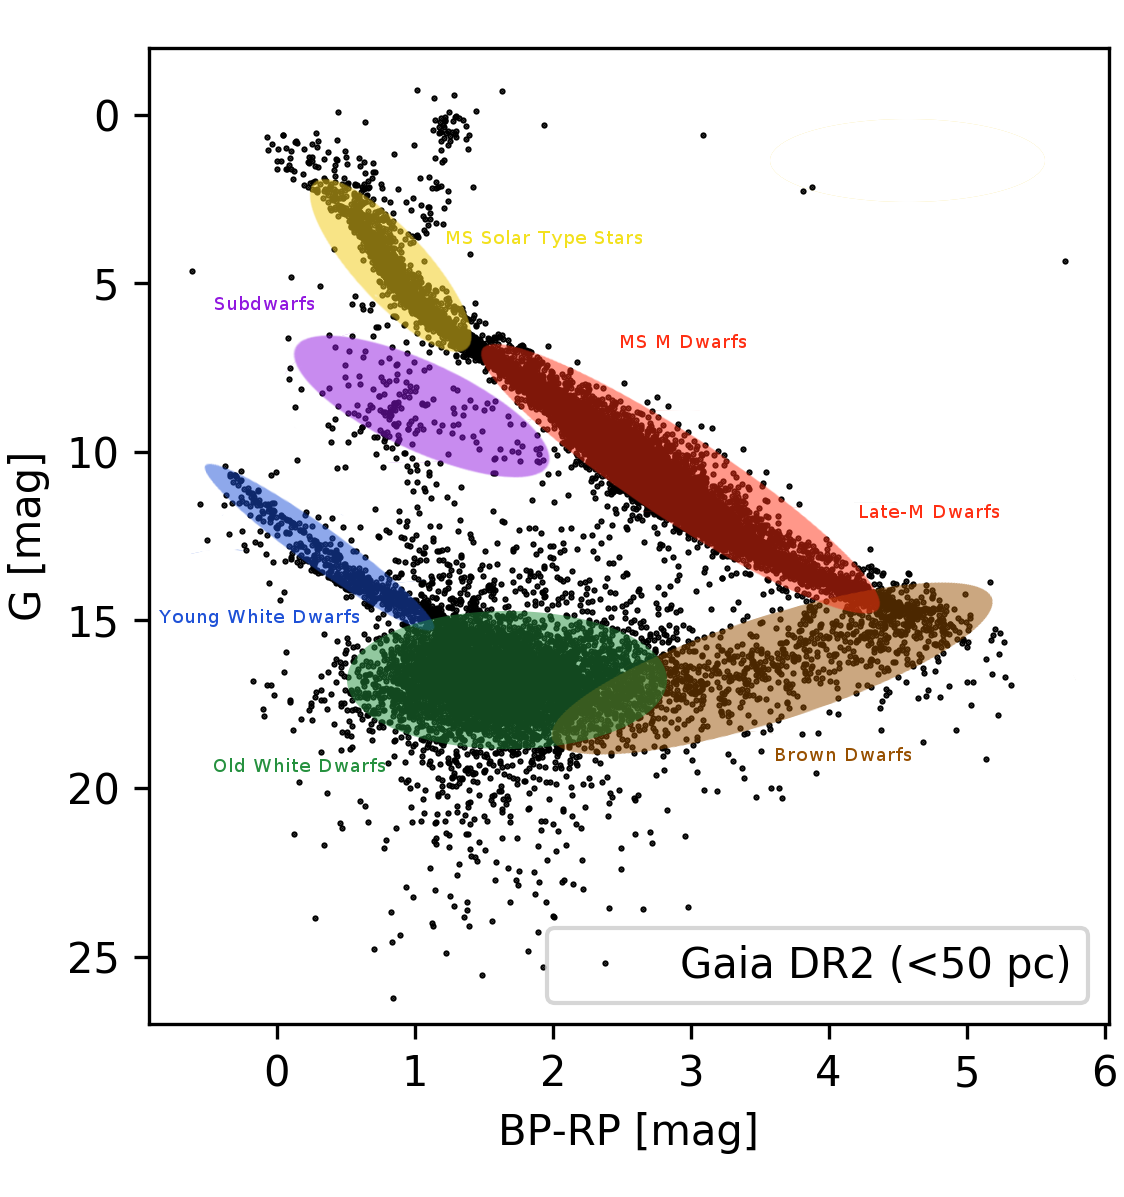
\includegraphics [scale=1.5] {gaia50types}
  \caption{На диаграмме <<показатель цвет $BP-RP$ -- абсолютная звездная величина в полосе G>> представлены звезды Gaia DR2 из ближайших окрестностей (до 50 пк). Цветными областями обозначено приблизительное разбиение звезд на группы, исходя из значений их показателей цвета и абсолютных звездных величин.}
  \label{fig:typ}
\end{figure}

\begin{figure}[pt]
  \centering
  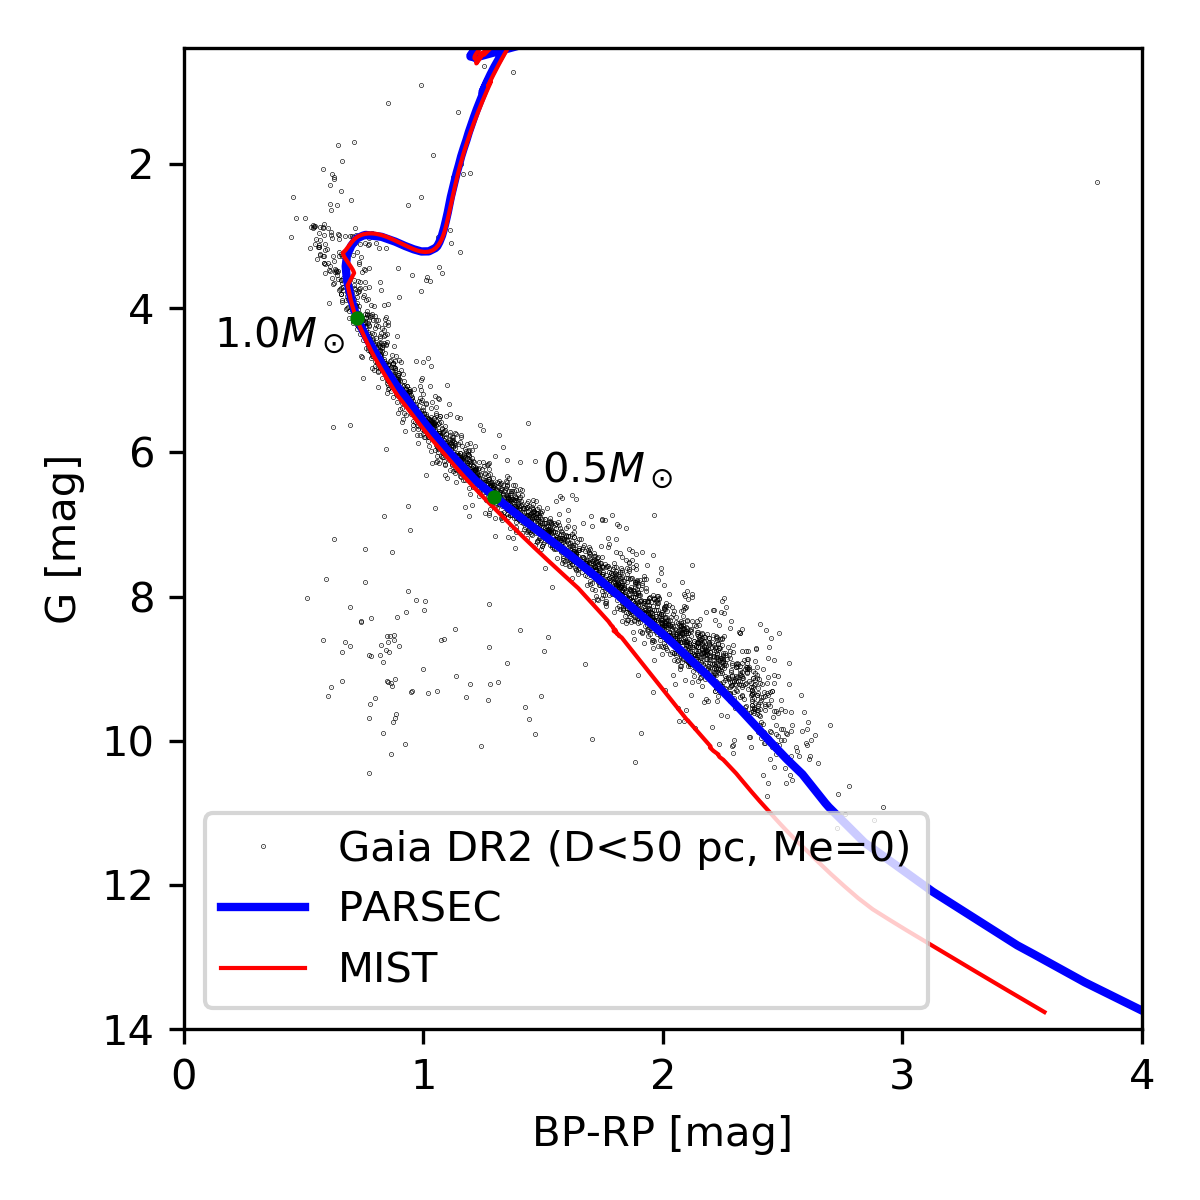
\includegraphics [scale=1.5] {parsec-mist-gaia}
  \caption{На диаграмме <<показатель цвет $BP-RP$ -- абсолютная звездная величина в полосе G>> представлены звезды Gaia DR2 из ближайших окрестностей (до 50 пк) с солнечной металличностью, соответствующие модельные изохроны проектов PARSEC и MIST, а также положения соответствующих звезд с массами 1 \(\textup{M}_\odot\) и 0.5 \(\textup{M}_\odot\).}
  \label{fig:iso}
\end{figure}

В настоящее время существует ряд проектов, нацеленных на конструирование моделей звезд различных типов. На рисунке~\ref{fig:iso} представлено сравнение звезд солнечной металличности из ближайших 50 пк по данным Gaia DR2 c модельными изохронами, построенными с помощью систем MIST \cite{2016ApJ...823..102C} и PARSEC \cite{2012MNRAS.427..127B}. Как видно из рисунка, для масс от 1 до 0.5 \(\textup{M}_\odot\) наблюдаемые данные очень хорошо согласуются с обеими изохронами, при массах менее 0.5 \(\textup{M}_\odot\) расхождение между системами изохрон весьма значительно, причем наилучшее согласие с наблюдениями имеет кривая, построенная с помощью PARSEC. Это можно объяснить в большей степени эмпирическим характером построения той части модели, которая описывает менее массивные звезды. Авторы PARSEC отмечают, что такой подход прежде всего связан с трудностью моделирования звездных атмосфер у объектов с сильным влиянием конвекционных процессов. Чтобы справиться с проблемой моделирования объектов легче, авторы PARSEC вносили поправки на основе данных для пары сотен наблюдаемых затменно-двойных звезд, для которых есть хорошие кривые лучевых скоростей (см. рисунок~\ref{fig:mrr}). Однако, выяснилось, что наблюдаемые затменно-двойные звезды слишком тесные, и соотношение масса-радиус для таких звезд не отвечает моделям одиночных звезд. Одно из предположений заключается в том, что в таких системах происходит инфляция радиуса за счёт взаимного нагрева компонент. Однако, попытка оценить такое влияние показала увеличение радиуса не более, чем на 6\,\%  при превосходстве светимости <<влияющего>> компаньона более, чем в 500 раз (см. рисунок~\ref{fig:inf}). Но эта работа продемонстрировала сложность физики взаимодействий в тесной системе маломассивных карликов, где имеют место  взаимные приливные деформации компонент. Поэтому крайне интересны двойные системы, состоящие из маломассивных звезд и при этом достаточно удаленные друг от друга, чтобы зависимость <<масса -- радиус>> соответствовала одиночным звездам. Собственно поиск таких систем и есть одна из целей настоящего исследования.

\begin{figure}[pt]
  \begin{minipage}[ht]{1\linewidth}\centering
    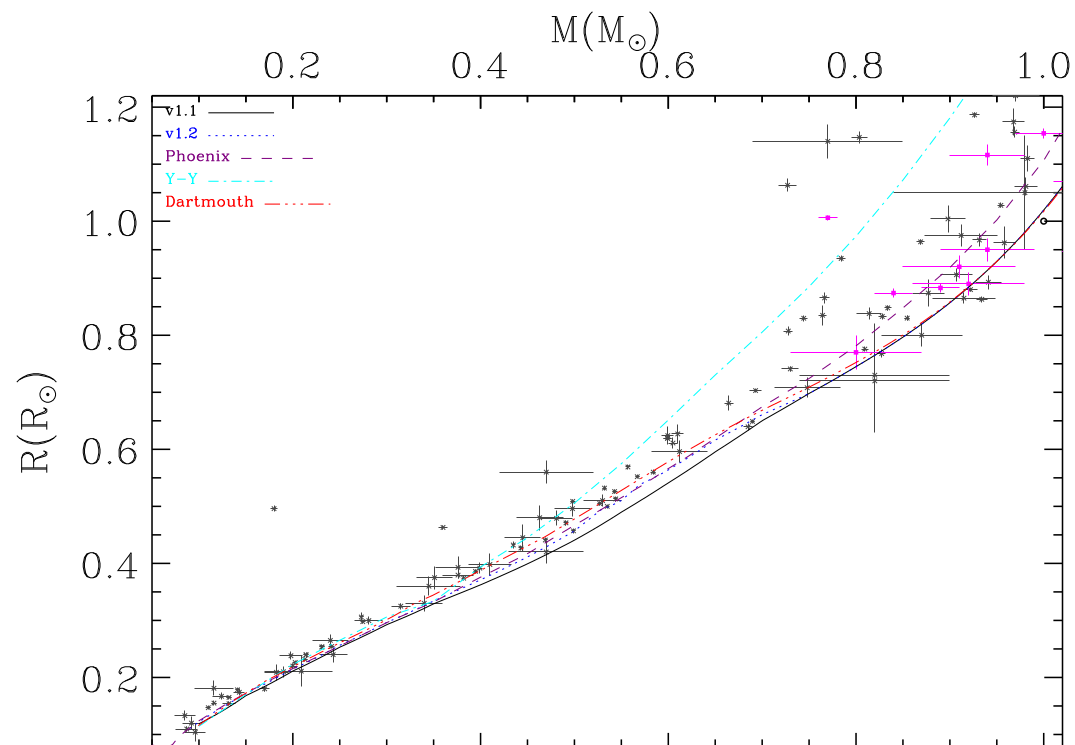
\includegraphics[width=0.8\linewidth]{parsecMRL1}% \\ а)
  \end{minipage}
  \hfill
  \begin{minipage}[ht]{1\linewidth}\centering
    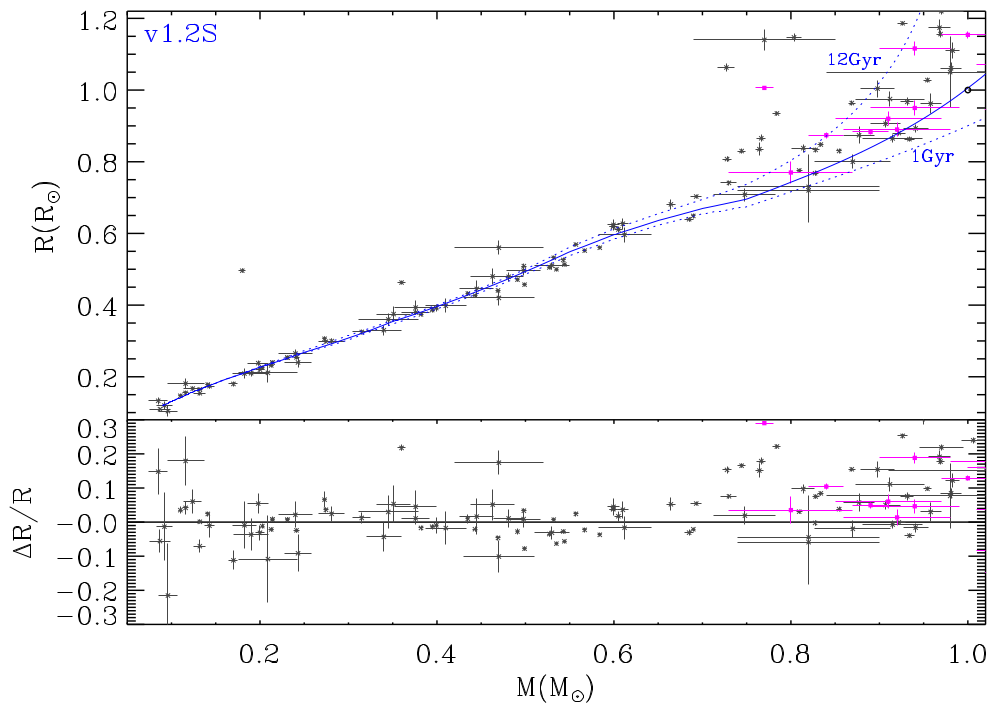
\includegraphics[width=0.8\linewidth]{parsecMRL2}% \\ б)
  \end{minipage}
  \caption{Сверху: эмпирическое отношение <<масса -- радиус>> для звезд с малой массой в солнечной окрестности. Черные звездочки "--- это двойные звезды; пурпурные квадраты "--- одиночные звезды. v1.1 и v1.2 "--- версии изохрон PARSEC (версия 1.2 "--- уточненная при помощи наблюдений нескольких сотен затменно-двойных, для которых есть хорошие кривые лучевых скоростей). Снизу: то же, только построенное для откалиброванного отношения <<T -- $\tau$>> (T "--- температура, $\tau$ "--- средняя оптическая глубина Росселанда) и с добавление изохрон для возрастов 1Gyr и 12Gyr. Взято из \cite{2014MNRAS.444.2525C}, рис. 2 и рис. 12).}
  \label{fig:mrr}
\end{figure}

\begin{figure}[pt]
  \centering
  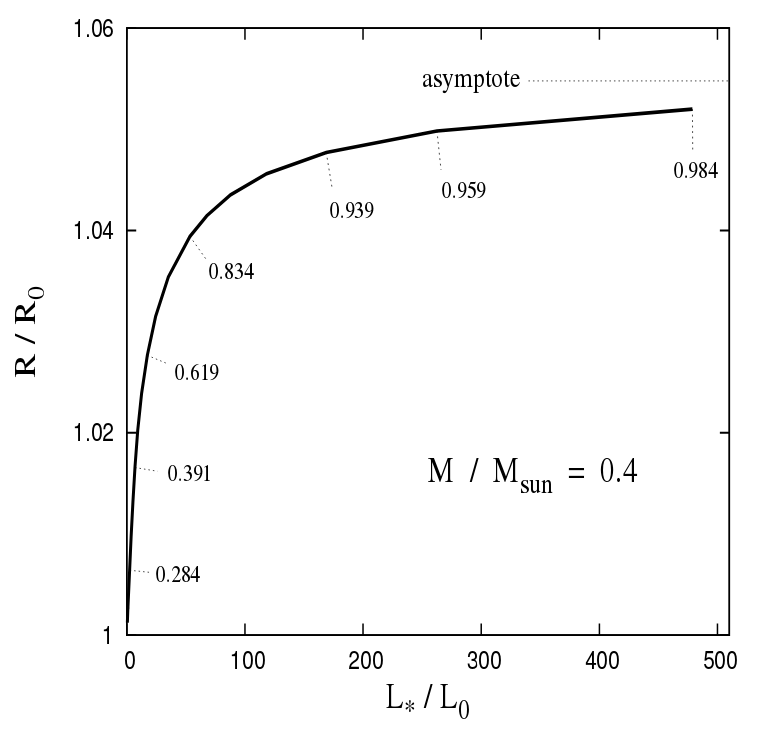
\includegraphics [scale=0.55] {radiusInflationLMSbinary}
  \caption{Попытка оценить влияние <<точечной>> компоненты затменно-двойной (a = 3 \(\textup{R}_0\)) со светимостью \(\textup{L}_*\) (отсечками на кривой показаны значения болометрического альбедо). Взято из \cite{2017A&A...601A..75L}, рис. 4.}
  \label{fig:inf}
\end{figure}

В качестве примера попытки построения эмпирической зависимости <<масса -- светимость>> (MLR) можно отметить работу \cite{2018MNRAS.479.5491E}, где использовались наблюдения звезд с наиболее надежными массами и светимостями. Всего в работу вошло 55 маломассивных объектов. На рисунке~\ref{fig:mlr} представлено сравнение этой модели с аналогичными кривыми по данным MIST и PARSEC, и как можно заметить, модели начинают расходиться при светимости меньше, а  объекты, наблюдаемые в пулковской программе изучения визуально-двойных звезд \cite{2018RAA....18...94S}, лежат у границ погрешностей эмпирической зависимости из работы \cite{2018MNRAS.479.5491E}, обозначенных пунктирной линией. Это тоже указывает на наличие дефицита надежных масс для звезд   M < 0.7~\(\textup{M}_\odot\). Поэтому калибровка существующих моделей карликовых звезд привязана к тесным системам, где оценки M и L могут быть искажены упомянутыми выше систематическими эффектами (несферичность, взаимный нагрев).

\begin{figure}[pt]
  \centering
  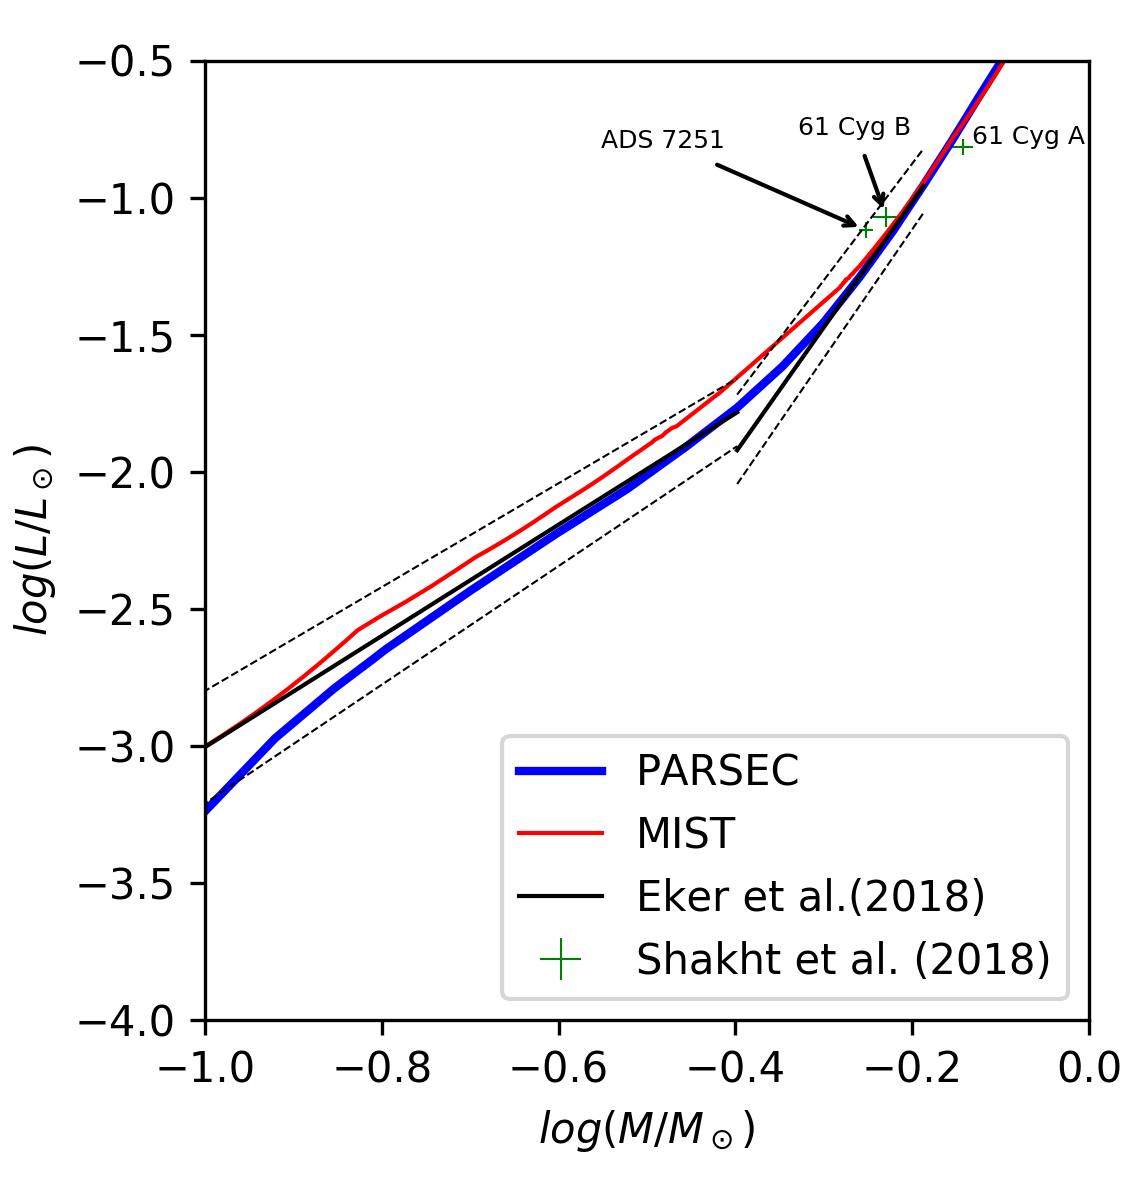
\includegraphics [scale=1.5] {mass-lum}
  \caption{Эмпирическая модель MLR \cite{2018MNRAS.479.5491E} (пунктиром обозначена граница ошибок модели), а также  аналогичные модели проектов PARSEC и MIST. Крестами обозначены визуально-двойные звезды из пулковской программы \cite{2018RAA....18...94S}.}
  \label{fig:mlr}
\end{figure}

Затронутая выше проблема учета конвекционных процессов в маломассивных звездах отмечается и в других работах. Например, в <<Обзоре маломассивных звезд и коричневых карликов>> \cite{2005astro.ph..9798C} говорится о сложности фотометрии звезд класса M5 и более поздних как раз из-за образования на поверхности большого числа звездных пятен и роста видимой активности диска и короны. Авторы объясняют это тем, что конвекция у таких объектов может распространяться вплоть до ядра.  Вообще, в данной работе говорится о целом наборе проблем, связанных с недостатком информации о карликах при их моделировании. На рисунке~\ref{fig:MLch} продемонстрировано, насколько хорошо существующие теоретические зависимости <<масса "--- абсолютная звездная величина>> согласуются с наблюдениями в оптическом диапазоне.

\begin{figure}[pt]
  \centering
  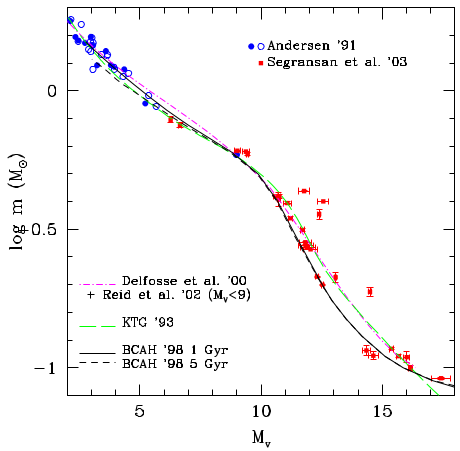
\includegraphics [scale=1.3] {chabrier-et-al-2005-3}
  \caption{Согласие теоретических моделей аналога зависимости <<масса -- звёздная величина>> с наблюдаемыми данными. Заметно расхождение теорий и наблюдений для звезд слабее 10 звездной величины и легче $\approx 0.5$\,\(\textup{M}_\odot\) (этому значению примерно соответствует отсчёт по вертикальной шкале около $-0.3$). Взято из \cite{2005astro.ph..9798C}, рис. 3.}
  \label{fig:MLch}
\end{figure}

Как можно заметить, для звёзд до \(\textup{10}^m\) согласие достаточно хорошее, тогда как более слабые объекты по диаграмме распределены несколько более хаотично и сильнее отклоняются от гладких модельных кривых. В статье говорится, что, вероятно, это связано с образованием большого количество линий поглощения. Исследователи отмечают, что в атмосферах маломассивных звёзд и коричневых карликов образуется множество молекул, чьи конденсаты и частицы сильно влияют на тепловую непрозрачность этих атмосфер. Излучение молекул часто поглощается в оптическом диапазоне или слишком слабо из-за эффекта обратного нагрева верхних слоев, где линии формируются. Всё это приводит к видимому покраснению звёзд, в частности, коричневые карлики излучают до 90\,\% своей энергии в ИК полосах, и авторы называют наиболее перспективными исследования данных объектов именно в этом диапазоне. Что согласуется с выводами авторов работы <<Необходимость инфракрасной астрометрии коричневых карликов в эпоху после Gaia>> \cite{2019BAAS...51c.105K}, которые указали на сложности наблюдений Gaia таких объектов. Исследователи отмечают, что диапазон наблюдений Gaia: $\lambda$ < 1,05 мкм \cite{2016A&A...595A...1G}, поэтому подавляющее большинство коричневых карликов, чьи спектры достигают максимума в ИК, не могут быть обнаружены. Например, в ближайших 20 парсеках Gaia может полностью исследовать только типы до L5 \cite{2019ApJS..240...19K}. И в материалах доклада проиллюстрирована необходимость астрометрического мониторинга на более длинных инфракрасных волнах.

Проблема надежного определения радиусов звёзд также упоминается в работе Шабрие \cite{2005astro.ph..9798C}. Отмечается, что используемые сейчас методы определения радиусов могут давать результаты, сильно отличающиеся друг от друга. Значения радиусов, определяемые через оценку наклона кривой блеска у затменных двойных получаются в среднем в 2 раза больше аналогичных радиусов, определенных высокоточной интерферометрией или через эффект гравитационного линзирования. Как уже отмечалось выше, это может быть связано с эффектом взаимного нагрева компонент слишком тесных систем.

Имеет смысл упомянуть об исследованиях по построению и интерпретации функции масс в окрестностях границы <<звёзды -- коричневые карлики>> \cite{2015ApJ...800...72T}. Здесь серьезное внимание уделяется проблеме адекватной оценки доли двойных систем для объектов малых масс. Функция масс претерпевает значимые изменения при разных значениях этой величины.  Это делает весьма актуальной задачу построения полной выборки двойных и кратных звезд в области малых масс. Наша работа имеет целью достичь продвижения в данном направлении.

Резюмируя вышеизложенное, естественно сделать вывод об актуальности исследования различных типов двойных и кратных систем карликовых звезд, в том числе "--- более широких, порядок периодов которых с одной стороны позволяет строить взаимные орбиты по высокоточным длительным наблюдениям, а с другой стороны "--- пространственное разделение компонент позволяло бы рассматривать каждую из компонент как одиночную звезду, без значительного влияния компаньона (большие полуоси у таких систем составляют порядка 10 а.е.). В современной научной печати можно найти многочисленные примеры работ, посвященных поиску двойных систем, разделению компонент и построению орбит двойных систем  (см., например, \cite{2015csss...18..805C}, \cite{2016ApJ...819...17O}).  

Построение численных моделей процесса звездообразования и дальнейшей динамической эволюции звездной популяции из молекулярных облаков позволяет получить модельные распределения доли двойных систем в зависимости от массы, отношения масс компонент и металличности, проанализировать различные распределения по орбитальным параметрам. Сопоставление результатов таких вычислений с наблюдениями затруднено неполнотой выборки для двойных систем, содержащих маломассивные компоненты. Это является еще одним обоснованием актуальности любых наблюдательных работ, направленных на поиск и изучение двойных и кратных систем среди карликовых звезд.

Сейчас можно найти немало исследований, посвященных построению численных сценариев звездообразования. Например, в работе \cite{2019MNRAS.484.2341B} представлен пример симуляции процесса формирования звездного скопления. Здесь учитывается масса факторов и явлений: химический состав межзвездной среды, влияние космических лучей, нагрев газа и пыли из-за излучения звезд, процессы диффузии и переноса излучения. В итоге модельное облако M = 500 \(\textup{M}_\odot\) порождает порядка сотни звезд суммарной массы $\approx$\,100~\(\textup{M}_\odot\) с медианной массой 0,15 \(\textup{M}_\odot\). Как видно из рисунка~\ref{fig:imf}, получившаяся функция масс наилучшим образом согласуется с результатами построения IMF \cite{2005ASSL..327...41C}, собравшим наблюдения маломассивных звезд и коричневых карликов на протяжении 50 лет.  Особое место в исследовании отведено изучению доли и свойств кратных объектов. Как следует из рисунка~\ref{fig:fract}, доля кратных систем в получившейся модели растёт с увеличением начальных масс объектов, и этот результат подтверждают и эмпирические данные. Причем исследователи отмечают, что так как доля кратных систем имеет явную корреляцию с значениями начальных масс, то при сравнении моделирования с наблюдениями всегда стоит использовать аналогичные диапазоны масс. На рисунке~\ref{fig:hist} представлено сравнение получившейся гистограммы распределения двойных, тройных и четверных систем по большим полуосям (тройные системы дают два значения полуосей, а четверные "--- три) с двумя эмпирическими построениями: для M-карликов и звезд с начальными массами солнечного типа. Отмечается, что поскольку большинство моделируемых объектов имеют малую массу, то ожидается, что распределение для M-карликов должно лучше соответствовать модели, и этот результат в большей мере воспроизводит гистограмма для двойных систем.  Попытка воссоздания эволюции доли двойных систем для кластеров звезд с различными начальными параметрами представлена, например, в работе \cite{2007ApJ...665..707H}. На рисунке~\ref{fig:evol} представлен результат моделирования эволюции доли двойных систем в кластере из 100~000 звезд, где в начальный заданный момент времени доля двойных составляла 10\,\%. Из рисунка видно, что с течением времени прогнозируемое моделью число кратных систем имеет явный тренд к возрастанию.

\begin{figure}[pt]
  \centering
  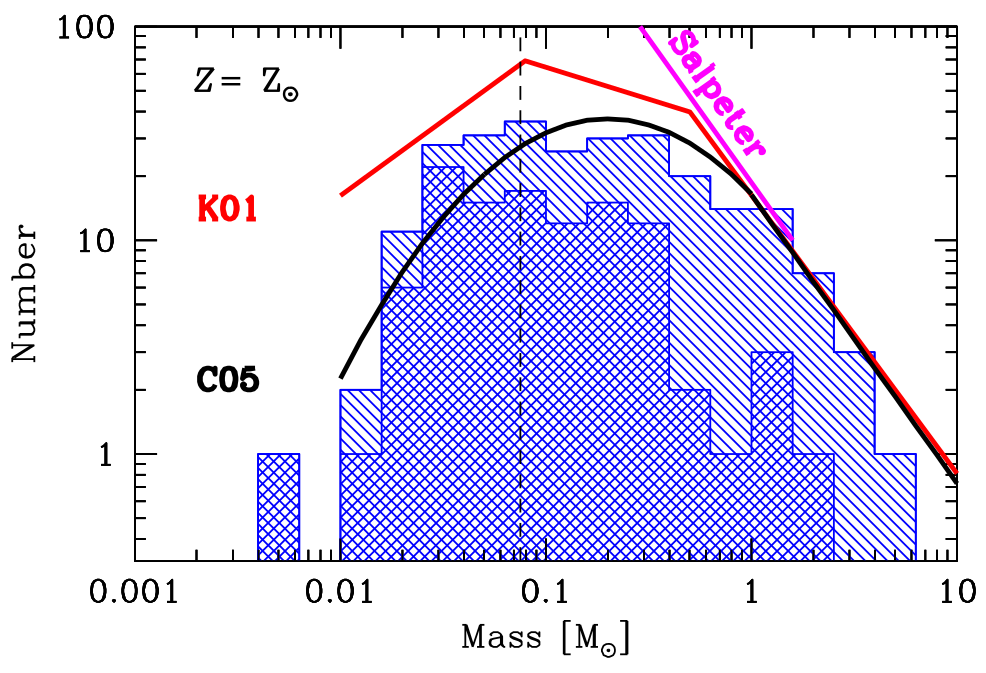
\includegraphics [scale=0.45] {Bate-IMF}
  \caption{Гистограмма IMF звезд и коричневых карликов солнечной металличности в рамках численной модели \cite{2019MNRAS.484.2341B}. Двойная штриховка "--- объекты без аккреции, одиночная штриховка "--- с аккрецией. Функции масс хорошо согласуются с данными \cite{2005ASSL..327...41C} (С05). Также представлены две другие IMF: Salpeter~\cite{1955ApJ...121..161S} и K01~\cite{2001MNRAS.322..231K}. Взято из \cite{2019MNRAS.484.2341B}, рис. 8, нижний левый.}
  \label{fig:imf}
\end{figure}

\begin{figure}[pt]
  \centering
  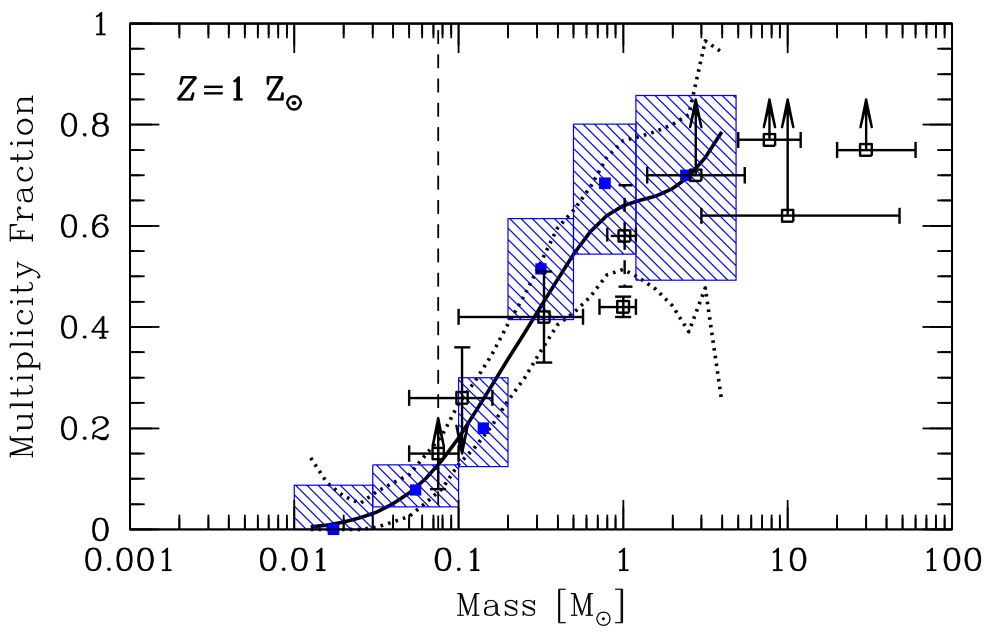
\includegraphics [scale=0.47] {Bate-BF}
  \caption{Доля кратности в зависимости от первичной массы звезд солнечной металличности в рамках численной модели \cite{2019MNRAS.484.2341B}. Синие закрашенные квадраты, окруженные заштрихованными областями, представляют результаты численных расчетов со статистической погрешностью 1$\sigma$. Толстая сплошная линия "--- кривая долей кратности, вычисленная с использованием скользящего логарифма, пунктирные линии "--- на 1$\sigma$-интервале вокруг нее. Незакрашенные квадраты с погрешностями и пределами "--- наблюдаемые доли кратных из исследований \cite{2003ApJ...587..407C}, \cite{2006AJ....132..663B}, \cite{1992ApJ...396..178F}, \cite{2010ApJS..190....1R}, \cite{1991A&A...248..485D}, \cite{2007A&A...474...77K}, \cite{2013MNRAS.436.1694R}, \cite{1999NewA....4..531P} и \cite{1998AJ....115..821M} слева направо.  Исследователи отмечают, что наблюдаемая тенденция увеличения кратности воспроизводится всеми рассмотренными расчетами, и поскольку доля кратных сильно зависит от начальных масс, важно, чтобы при сравнении моделей с наблюдениями использовались аналогичные массы. Взято из \cite{2019MNRAS.484.2341B}, рис. 10, нижний левый.}
  \label{fig:fract}
\end{figure}

\begin{figure}[pt]
  \centering
  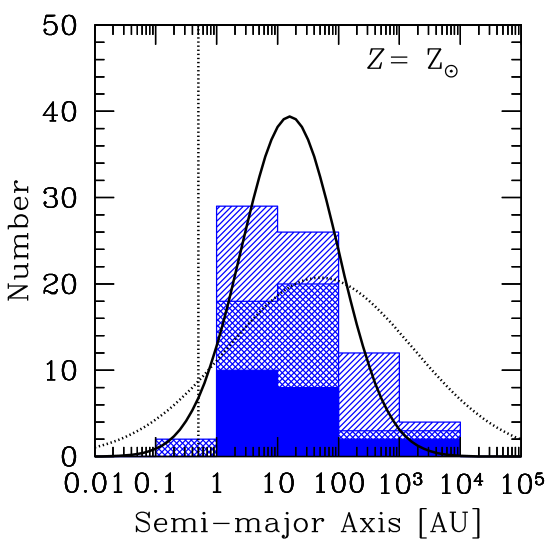
\includegraphics [scale=0.8] {Bate-a-distr}
  \caption{Гистограмма распределения кратных звезд солнечной металличности с начальными массами > 0.1Msun по большим полуосям в рамках численной модели \cite{2019MNRAS.484.2341B}.  Бары с одиночной, двойной и сплошной штриховкой представляют двойные, тройные и четверные системы соответственно. Сплошная кривая "--- распределение M-карликов из обзора \cite{2012ApJ...754...44J}, а пунктирная "--- распределение звезд с начальными массами солнечного типа из обзора \cite{2010ApJS..190....1R}. Поскольку большинство моделируемых систем имеют малую массу, ожидается, что распределение \cite{2012ApJ...754...44J} будет соответствовать лучше, чем \cite{2010ApJS..190....1R}. Вертикальная пунктирная линия показывает предел разрешающей способности расчетов, который определяется радиусами аккреции поглощающих частиц (0,5 а.е.). Взято из \cite{2019MNRAS.484.2341B}, рис. 11, третий слева.}
  \label{fig:hist}
\end{figure}


\begin{figure}[pt]
  \centering
  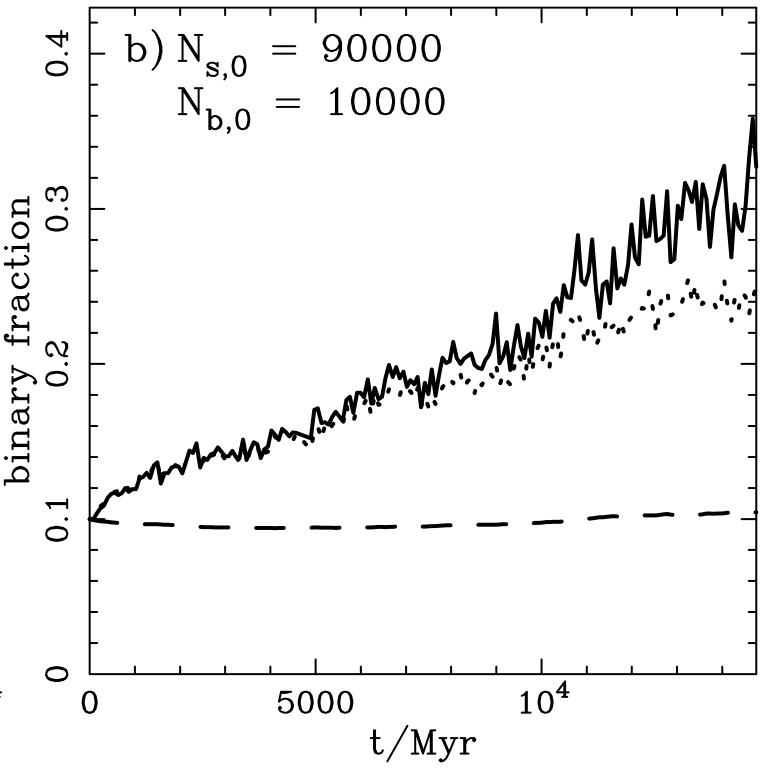
\includegraphics [scale=0.5] {Hurley}
  \caption{Эволюция доли двойных систем в ядре (сплошная линия), в пределах 10\,\% радиуса Лагранжа (пунктирная линия) и для всего кластера (пунктирная линия) в одной из моделей. $N_{s,0}$, $N{b,0}$ "---  количества одинарных и двойных звезд соответственно в исходной модели.  Взято из \cite{2007ApJ...665..707H}, рис. 7b.}
  \label{fig:evol}
\end{figure}

Однако, пока сложно утверждать, что даже совокупность существующих обзоров и программ решает проблему в полной мере. К сожалению, несмотря на существенный прогресс в исследовании кратных систем, который дает Gaia DR2, даже после значительного исправления первого релиза, данные миссии также не дают полноты выборки для визуальных двойных звезд с разделением $\rho$ менее $2''$ (рисунок~\ref{fig:compl}), что отмечают и авторы \cite{2018A&A...616A..17A},\cite{2018A&A...616A...2L}. Это может быть связано со сложностью анализа изображения тесных систем в Gaia DR2 \cite{2016A&A...595A...3F}, когда FWHM (ширина на полувысоте) становится меньше углового разделения $\rho$ (см. рисунок~\ref{fig:spf}). Сложность разделения тесных систем сказывается и на ошибках определения пиксельных координат, что в свою очередь влияет на вычисляемые значения собственных движений и параллаксов. Например, на рисунке~\ref{fig:err} можно увидеть, как относительная точность параллаксов Gaia DR2 падает при $\rho$~<~$2''$. Кроме того, отмечается проблема кросс-идентификации быстрых объектов ($\mu$~>~100 mas/yr), которые в основном как раз относятся к ближайшему звездному населению. Как указано в GaiaDR2 Documentation 1.2\footnote{\textit{https://gea.esac.esa.int/archive/documentation/GDR2/index.html}}, для звезд с разделением менее $0.7''$ всегда будет стоять проблема кросс-идентификации, и поэтому объекты Gaia DR2 с флагом <<duplicate source>> предлагается отдельно проверять, являются ли они действительно дубликатами одиночной звезды или же входят в двойную или кратную систему. Помимо проблемы отождествления тесных объектов, стоит упомянуть, что период наблюдений миссии Gaia строго ограничен и не дает возможности получения достаточного количества наблюдений для построения орбит широких пар, периоды взаимного обращения которых сильно превалируют над сроком жизни космического аппарата.

\begin{figure}[pt]
  \centering
  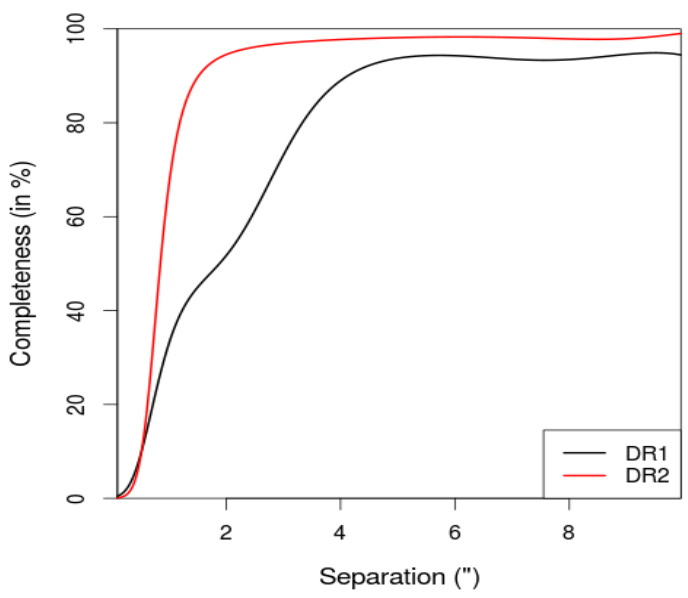
\includegraphics [scale=0.6] {gaia-complitness-for-binaries}
  \caption{Полнота (\%) визуальных двойных звёзд из каталога WDS в зависимости от разделения между компонентами (WDS), детектируемых в ходе миссии Gaia.  Gaia DR1 (черный), Gaia DR2 (красный). Заметно снижение полноты выборки двойных для тесных систем ($\rho$ < 2 arcsec). Взято из \cite{2018A&A...616A..17A}, рис. 8.}
  \label{fig:compl}
\end{figure}

\begin{figure}[pt]
  \centering
  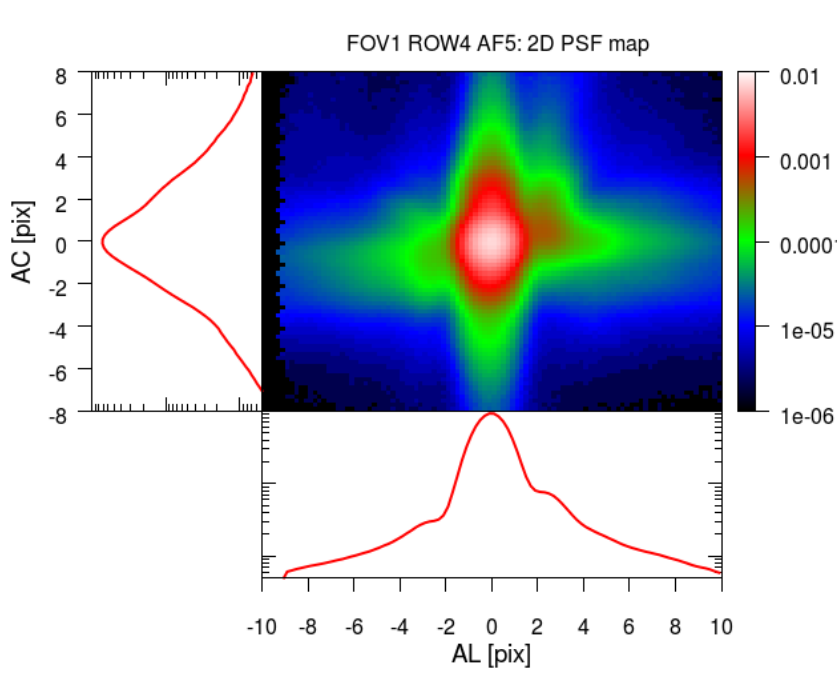
\includegraphics [scale=0.6] {gaia-psf}
  \caption{PSF изображения тесной двойной (1.2$''$ на 2.8$''$) демонстрирует сложность разделения в Gaia DR2 изображений подобных звезд. Взято из \cite{2016A&A...595A...3F},  рис. 7.}
  \label{fig:spf}
\end{figure}

\begin{figure}[pt]
  \centering
  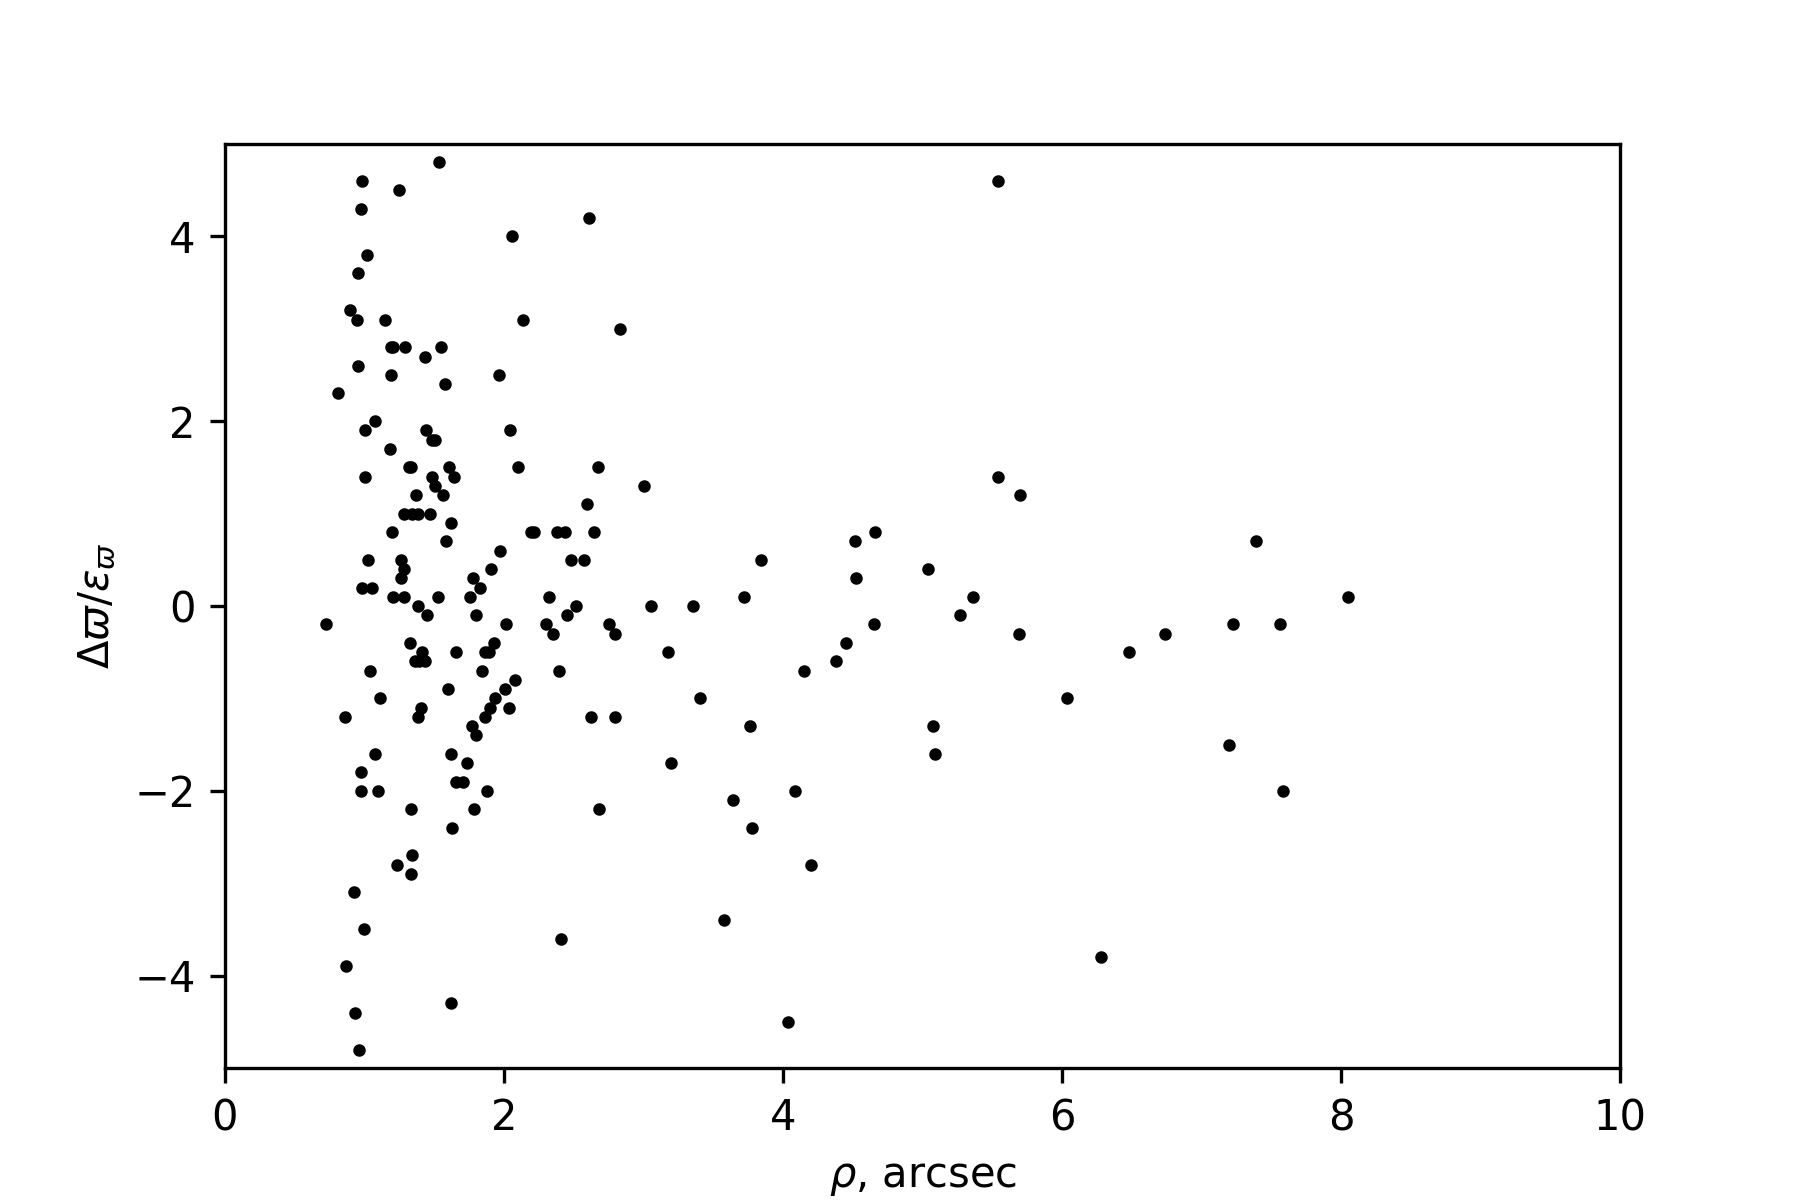
\includegraphics [scale=1.2] {delta_pi-vs-rho}
  \caption{Увеличение разброса относительных ошибок параллаксов Gaia для изображений звезд с разделением менее 3$''$ указывает на существенное снижение точности определения пиксельных координат компонент.}
  \label{fig:err}
\end{figure}

В связи с указанными проблемами важным становится применение всех доступных методик детектирования кратности звезд и использование по возможности всех доступных наблюдений звезд, охватывающих широкий диапазон эпох. Исследования звезд в ближайших 50 пк от Солнца дают возможность наиболее эффективного их применения. Как можно убедиться из рисунка~\ref{fig:sepdis}, для звездных систем с величинами больших полуосей порядка 10 а.е. видимое разделение компонент даже в ближайшем окружении составляет меньше $1''$. К счастью, существующие методы высокого разрешения (спекл-интерферометрия, метод удачных экспозиций) позволяют разделять объекты $\rho$~<~$1''$ (см. рисунок~\ref{fig:lucky}). Однако данные методы сложно применять массово, так как требуют таргетированных и часто многочисленных наблюдений, и больше подходят для построения орбит уже выявленных двойных и кратных систем.

\begin{figure}[pt]
  \centering
  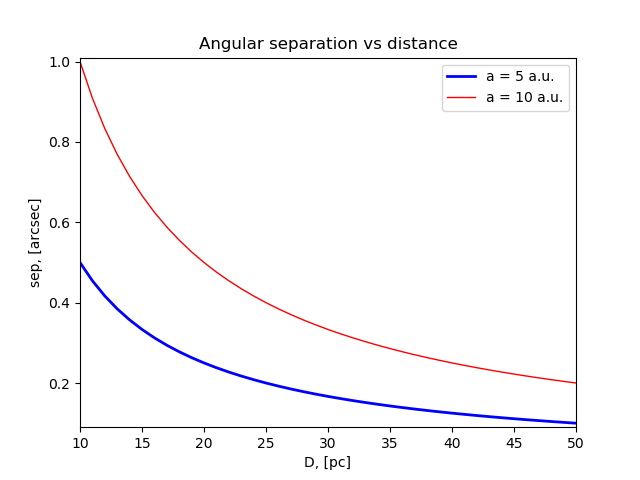
\includegraphics [scale=1.1] {separation-vs-distance}
  \caption{Представлена зависимость от удаления видимого углового разделения компонент систем с заданными большими полуосями. Поиск и определение динамических параметров маломассивных двойных систем "--- актуальная задача, требующая наблюдений широкого класса объектов, для которых разделение $\rho$~<~FWHM.}
  \label{fig:sepdis}
\end{figure}

\begin{figure}[pt]
  \centering
  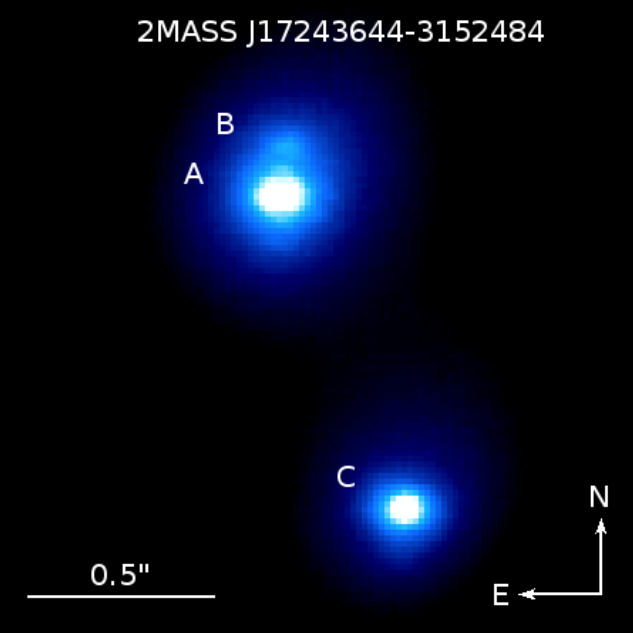
\includegraphics [scale=0.6] {lucky-imaging-example}
  \caption{Рис 15. 3.5m New Technology Telescope (NTT) "--- метод удачных экспозиций (Lucky imaging). Взято из \cite{2017A&A...599A..70J}, рис. 1. }
  \label{fig:lucky}
\end{figure}

Близость исследуемых объектов позволяют эффективно применять различные методы современной астрономии для их изучения. Например, наиболее заметные смещения компонент близких систем по лучу зрения дают возможность плодотворно выявлять оптически неразрешаемые спектрально-двойные звезды благодаря значительному проявлению эффекта доплеровского смещения спектральных линий. Однако, объектами таких исследований становятся в основном всё те же тесные системы, массы и радиусы которых сложно использовать для построения моделей одиночных звезд.

Целью данной работы является разработка метода поиска двойных и кратных звезд, дальнейшее определение орбитальных параметров которых позволят получить более надежные массы, радиусы и светимости маломассивных звезд и коричневых карликов и уточнить фундаментальные закономерности для этих групп объектов. Исследуемые системы преимущественно должны быть не слишком тесными, чтобы компоненты не влияли в значительной мере на характеристики друг друга, а их периоды составляли несколько десятилетий, что дает возможность построить орбиту по короткой дуге за относительно небольшой отрезок времени. Поэтому объектами наших поисков являются двойные звезды низкой светимости из ближайшего окружения Солнца, большие полуоси взаимных орбит которых составляют примерно 5--10 а.е.. Как уже отмечалось, даже в ближайшей солнечной окрестности такие системы часто разрешимы только  с помощью наблюдений методами высокого разрешения  (спекл-интерферометрия, метод удачных экспозиций), которые нельзя использовать для массовых наблюдений. Поэтому одна из задач данного исследования состоит в разработке методов обнаружения искомых двойных систем, основанных на подходах традиционной наземной оптической астрометрии и анализа изображений.

Актуальность рассматриваемых проблем способствовала тому, что в XX в. было реализовано несколько проектов, направленных на обнаружение быстрых звезд \cite{1955AJ.....60..274D}, \cite{1979nlcs.book.....L} и на определение их собственных движений и тригонометрических параллаксов \cite{1995gcts.book.....V}. Научные группы из различных обсерваторий прилагают усилия в этом направлении. Большой цикл работ по данной тематике представляет команда проекта RECONS (см., например, \cite{2017AJ....153...14W}), имеются существенные результаты в рамках проекта MEarth \cite{2017ApJ...836..124D}. Часть исследований в рамках пулковской программы по изучению звезд с большими собственными движениями имела целью детектирование двойных систем, о чем свидетельствует цикл работ: \cite{2011AstL...37..420K}, \cite{2015AstL...41..833K}, \cite{2016AstL...42..686K}.

\newpage

Подводя итог вводной части работы коротко резюмируем основные моменты.
% {\progress}
% Этот раздел должен быть отдельным структурным элементом по
% ГОСТ, но он, как правило, включается в описание актуальности
% темы. Нужен он отдельным структурынм элемементом или нет ---
% смотрите другие диссертации вашего совета, скорее всего не нужен.

{\aim} данной работы является выявление двойных систем среди близких к Солнцу маломассивных карликовых звезд. 

Для~достижения поставленной цели необходимо было решить следующие {\tasks}:
\begin{enumerate}
  \item Оценить полноту современных обзоров и списков двойных систем;
  \item Сформировать список звезд для исследования;
  \item Разработать методы быстрого и массового поиска двойных систем среди близких к Солнцу маломассивных карликов, основанных на подходах наземной оптической астрометрии и анализа цифровых изображений звездообразных объектов.
\end{enumerate}

Актуальность данного исследования обусловлена недостатком надежных оценок масс для карликовых звезд, затрудняющим построение их физических моделей с одной стороны, и необходимостью верификации численных моделей формирования звездных популяций, в которой важную роль играют эмпирические распределения двойных систем по ряду параметров, с другой стороны.

{\novelty}
\begin{enumerate}
  \item Были предложены новые варианты методик поиска двойных систем на основе анализа собственных движений и путем анализа формы изображений звезд на ПЗС-кадрах;
  \item Выполнены собственные ПЗС-наблюдения, позволившие произвести проверку адекватности разработанных методов и выявить 259 звезд-кандидатов в двойные системы;
  \item В результате спекл-интерферометрических наблюдений на БТА САО РАН и 2.5 м телескопе КГО ГАИШ МГУ впервые детектирована двойственность систем J1158+4239, J1135+0414, J1147+6050, независимо подтверждены ранее уже выявленные двойные звезды J1601+3714, J0259+3636.
\end{enumerate}

Теоретическая значимость работы определяется модификацией метода Вилена, позволяющей выявлять двойственность звезд на основе анализа собственных движений на основе ПЗС-кадров и сканов фотопластинок с общей системой опорных звезд; адаптацией шейплет-формализма для оценивания эллиптичности и асимметрии звездных изображений на ПЗС-кадрах.

{\influence} состоит в проведении большого цикла астрономических наблюдений на Нормальном астрографе и метровом телескопе «Сатурн» в Пулковской обсерватории, анализ результатов которого позволил выявить двойственность упомянутых выше звезд. Важно, что представленные методы реализованы в виде программного обеспечения, которое может быть адаптировано для других инструментов различных обсерваторий.

{\methods} За основу исследований были взяты зарекомендовавшие себя технологии исследования быстрых звезд ($\Delta\mu$-двойные) и анализа изображений (shapelet-декомпозиция), которые были адаптированы с учетом исследуемого материала и успешно применены для поиска двойных звезд среди близких карликов.

{\defpositions}
\begin{enumerate}
  \item Модификация метода Вилена по выявлению звезд-кандидатов в $\Delta\mu$-двойные;
  \item Адаптация шейплет-формализма для детектирования скрытых двойных звездных изображений;
  \item Выявление 259 звезд--кандидатов в маломассивные двойные системы;
  \item Подтверждение двойственности пяти систем методами высокого разрешения.
\end{enumerate}


{\reliability} полученных результатов обеспечивается частичным присутствием найденных двойных звезд в существующих каталогах двойных звезд, в том числе "--- WDS.


{\probation}
Детальное изложение методов и результатов работы представлено в четырех публикациях, индексируемых в наукометрических базах данных (web of science, Scopus и т.п.), в устных докладах на российских и международных конференциях (астрометрические конференции <<Пулково--2012>>, <<Пулково--2015>>, <<Пулково--2018>>; ВАК--2013 (Санкт-Петербург); ВАК--2016 (Нижний Архыз); <<Современная астрометрия>> (Москва)), астрометрических семинарах Пулковской обсерватории и Пулковских молодежных конференциях. Кроме того, результаты исследований доступны в астрономических базах данных (CDS, WDS).
%\textbf{Публикации.} Основные результаты по теме диссертации изложены в 4 печатных изданиях. Из них 3 изданы в журналах, рекомендованных ВАК, 4 индексируются в Scopus (1 работа является материалами конференции), 3 индексируются в Web of Science. 

{\contribution} Автор принимал активное участие во многих этапах работы: наблюдения на пулковских  телескопах (Нормальном астрографе и телескопе <<Сатурн>>), написание программного обеспечения для вычисления и анализа собственных движений звезд, написание текстов для совместных с соавторами научных статей, выступления на научных конференциях с устными докладами, посвященными настоящему исследованию. 


%\ifnumequal{\value{bibliosel}}{0}
{%%% Встроенная реализация с загрузкой файла через движок bibtex8. (При желании, внутри можно использовать обычные ссылки, наподобие `\cite{vakbib1,vakbib2}`).
    %{\publications}% Основные результаты по теме диссертации изложены в XX печатных изданиях,
    %X из которых изданы в журналах, рекомендованных ВАК,
    %X "--- в тезисах докладов.
}% 
{%%% Реализация пакетом biblatex через движок biber
    %\begin{refsection}[bl-authorvak,bl-authorwos,bl-authorscopus,bl-authorother,bl-authorconf]
        % Это refsection=1.
        % Процитированные здесь работы:
        %  * подсчитываются, для автоматического составления фразы "Основные результаты ..."
        %  * попадают в авторскую библиографию, при usefootcite==0 и стиле `\insertbiblioauthor` или `\insertbiblioauthorgrouped`
        %  * нумеруются там в зависимости от порядка команд `\printbibliography` в этом разделе. 
        %  * при использовании `\insertbiblioauthorgrouped`, порядок команд `\printbibliography` в нём должен быть тем же (см. biblio/biblatex.tex)
        %
        % Невидимый библиографический список для подсчёта количества публикаций:
        %\printbibliography[heading=nobibheading, section=1, env=countauthorvak,    keyword=biblioauthorvak]%
        %\printbibliography[heading=nobibheading, section=1, env=countauthorwos,    keyword=biblioauthorwos]%
        %\printbibliography[heading=nobibheading, section=1, env=countauthorscopus, keyword=biblioauthorscopus]%
        %\printbibliography[heading=nobibheading, section=1, env=countauthorconf,   keyword=biblioauthorconf]%
        %\printbibliography[heading=nobibheading, section=1, env=countauthorother,  keyword=biblioauthorother]%
        %\printbibliography[heading=nobibheading, section=1, env=countauthor,       keyword=biblioauthor]%
        %
        % Цитирования.
        %  * Порядок перечисления определяет порядок в библиографии (только внутри подраздела, если `\insertbiblioauthorgrouped`).
        %  * Если не соблюдать порядок "как для \printbibliography", нумерация в `\insertbiblioauthor` будет кривой.
        %  * Если цитировать каждый источник отдельной командой --- найти некоторые ошибки будет проще.
        %
        %% authorvak
        %\nocite{vakbib1}%
        %\nocite{vakbib2}%
        %\nocite{vakbib3}
        %
        %% authorwos
        %\nocite{wosbib1}%
        %
        %% authorscopus
        %\nocite{scbib1}%
        %
        %% authorconf
        %\nocite{confbib1}%
        %\nocite{confbib2}%
        %
        %% authorother
        %\nocite{bib1}%
        %\nocite{bib2}%
        %\nocite{bib3}
        %\nocite{bib4}
        %\nocite{bib5}
        %
        %
        %{\publications} Основные результаты по теме диссертации изложены в~\arabic{citeauthor}~печатных изданиях,
        %\newcounter{citeauthorscwostot}% сумма citeauthorscopus и citeauthorwos
        %\setcounter{citeauthorscwostot}{\value{citeauthorscopus}}%
        %\addtocounter{citeauthorscwostot}{\value{citeauthorwos}}%
        %\arabic{citeauthorvak} из которых изданы в журналах, рекомендованных ВАК\sloppy%
        %\ifnum \value{citeauthorscwostot}>0%
        %    , \arabic{citeauthorscwostot} "--- в~периодических научных журналах, индексируемых Web of Science и Scopus\sloppy%
        %\fi%
        %\ifnum \value{citeauthorconf}>0%
        %    , \arabic{citeauthorconf} "--- в~тезисах докладов.
        %\else%
        %    .
        %\fi
    %\end{refsection}%
    %\begin{refsection}[bl-authorvak,bl-authorwos,bl-authorscopus,bl-authorother,bl-authorconf]
        % Это refsection=2.
        % Процитированные здесь работы:
        %  * попадают в авторскую библиографию, при usefootcite==0 и стиле `\insertbiblioauthorimportant`.
        %  * ни на что не влияют в противном случае
        %\nocite{vakbib2}%vak
        %\nocite{bib1}%other
        %\nocite{confbib1}%conf
    %\end{refsection}%
	%
	% Всё, что вне этих двух refsection, это refsection=0,
	%  * для диссертации - это нормальные ссылки, попадающие в обычную библиографию
	%  * для автореферата:
	%     * при usefootcite==0, ссылка корректно сработает только для источника из `external.bib`. Для своих работ --- напечатает "[0]" (и даже Warning не вылезет).
	%     * при usefootcite==1, ссылка сработает нормально. В авторской библиографии будут только процитированные в refsection=0 работы.
}
 % Характеристика работы по структуре во введении и в автореферате не отличается (ГОСТ Р 7.0.11, пункты 5.3.1 и 9.2.1), потому её загружаем из одного и того же внешнего файла, предварительно задав форму выделения некоторым параметрам

%Диссертационная работа была выполнена при поддержке грантов ...

%\underline{\textbf{Объем и структура работы.}} Диссертация состоит из~введения,
%четырех глав, заключения и~приложения. Полный объем диссертации
%\textbf{ХХХ}~страниц текста с~\textbf{ХХ}~рисунками и~5~таблицами. Список
%литературы содержит \textbf{ХХX}~наименование.

\section*{Содержание работы}
Во \underline{\textbf{введении}} обосновывается актуальность
исследований, проводимых в~рамках данной диссертационной работы,
приводится обзор научной литературы по изучаемой проблеме,
формулируется цель, ставятся задачи работы, излагается научная новизна
и практическая значимость представляемой работы. В~последующих главах
сначала описывается исторический опыт и общий принцип, позволяющий детектировать астрометрические двойные, прошлая реализация метода, а~потом идёт описание адаптации описанного метода, реализация данной адаптации, верификация проводимых исслдеований и приведены результаты: впервые открытые двойные и кратные звезды.


\underline{\textbf{Первая глава}} посвящена освещению прошлого опыта реализаций астрометрического подхода для нахождения двойных и кратных систем. 

В первой части главы приводится краткая историческая справка об изучении быстрых звезд, реализации первой космической астрометрической программы Hipparcos. 

Во второй части дано подробное описание ставшего основой данной работы метода Вилена \cite{1999A&A...346..675W} для нахождения двойных звезд через статистические исследования колебаний значений собственных движений неразрешаемых систем, основная идея которого представлена на рис.~\ref{fig:widea}.
\begin{figure}[ht]
 \centering
 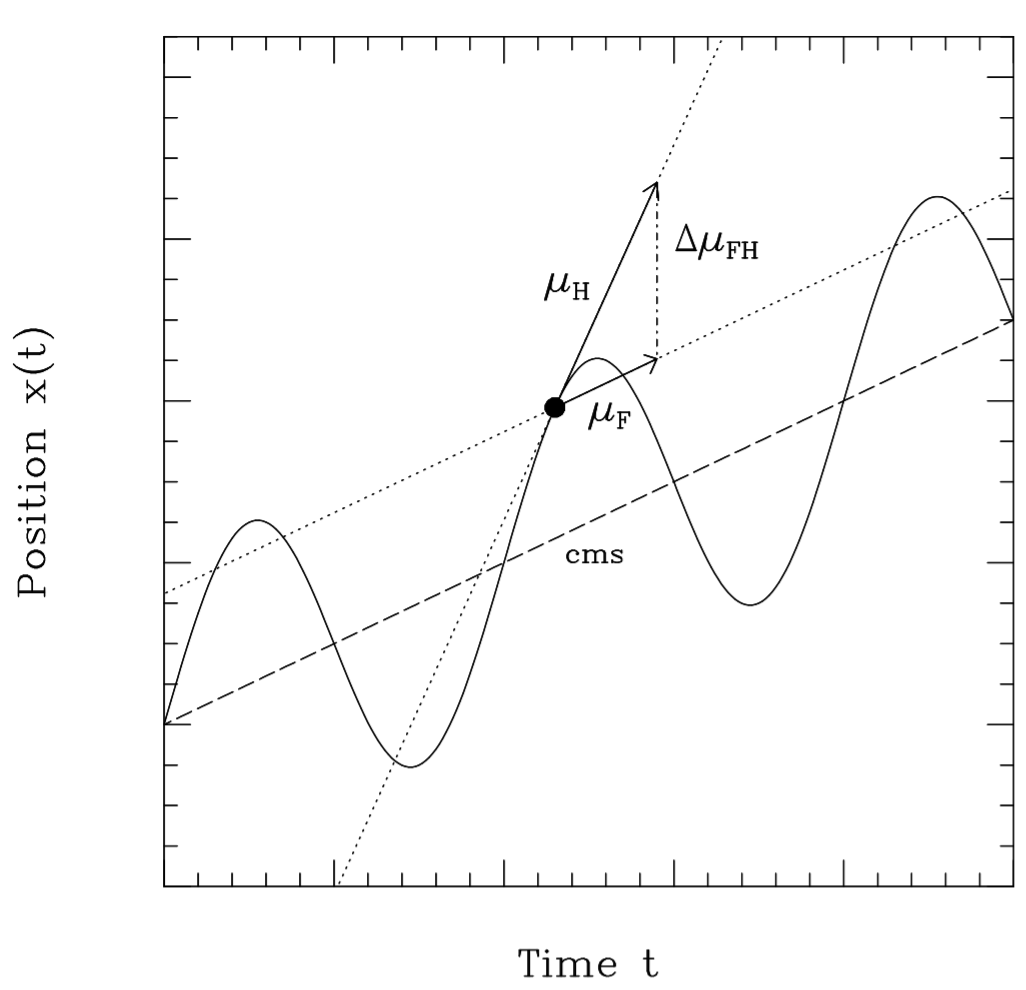
\includegraphics [width=0.7\linewidth] {Wielen-idea}
 \caption{Колебания фотоцентра двойной системы, вызванные влиянием орбитального движения, приводит к заметной разнице $\Delta\mu_{FH}$ между мгновенно измеренным собственным движением Hipparcos $\mu_{H}$ и средним собственным движением $\mu_{F}$ фотоцентра. Здесь период обращения двойной системы имеет среднюю длину ($\approx$\,30 лет), так что собственное движение $\mu_{F}$, полученное из наземных данных (например, из FK5), по существу равно собственному движению барицентра (cms) двойной звезды. Взято из \cite{1999A&A...346..675W}, Рис.~1.}
 \label{fig:widea}
\end{figure}

В работе \cite{1999A&A...346..675W} рассматривались ярчайшие звезды миссии Hipparcos, исследовалась статистическая значимость по отношению к ошибкам разностей квазимгновенных собственных движений, полученных в ходе космической миссии, и квазисредних собственных движений, рассчитанных на основе наиболее ранних положений звезд, полученных из каталогов GC и FK5. Статистическая значимость разностей положений (после ввода некоторых поправок для исключения корелляций компонент собственных движений) выражалась формулой~\ref{eq:WiF}.
\begin{equation}
  \label{eq:WiF}
  F^{2}_{0H} =\left(\frac{\Delta\mu_{0H,\psi}}{\epsilon_{\Delta\mu_{0H,\psi}}}\right)^{2}+\left(\frac{\Delta\mu_{0H,\bar{\psi}}}{\epsilon_{\Delta\mu_{0H,\bar{\psi}}}}\right)^{2}.
\end{equation}
Параметр $F$ отображает статистическую значимость разностей квазисреднего и квазимгновенного собственных движений $\Delta\mu$ по отношению к ошибкам их определения $\epsilon_{\Delta\mu}$. Пороговые значения параметра в работе 1999 года были определены как $F>3.44$ для $\Delta\mu$-двойных звезд и $F<2.49$ для кандидатов в одиночные звезды.

Третья часть первой главы разделена на 3 пункта и в целом дает оценку состоятельности рассматриваемой задачи поиска $\Delta\mu$-двойных звезд среди близких карликов. В первом пункте рассматриваются некоторые свойства видимых орбит фотоцентров маломассивных двойных систем, в частности, отмечается, что нелинейность движения фотоцентра маломассивных систем на определенном расстоянии можно обнаружить практически всегда, за исключением только, пожалуй, случаев равенства масс и светимостей компонент. Во втором пункте приведена оценка количества $\Delta\mu$-двойных среди близких карликов. По результатам исследования модельной популяции маломассивных звезд, построенной с привлечением функции масс из работы \cite{2005ASSL..327...41C}, распределения больших полуосей из статьи \cite{2010ApJS..190....1R}, а также подсчетов звезд в солнечной окрестности, произведенных коллаборацией RECONS \cite{2019AJ....157..216W} и другими авторами на основе данных Gaia DR2, оценка количества $\Delta\mu$-двойных по всему небу оказалась примерно 1000 звезд, в Пулковской зентиной зоне ($30^\circ$ -- $70^\circ$) "--- около 250 объектов. В четвертом пункте третьей части первой главы дана оценка количества маломассивных кратных звездных систем, выявляемых через оценку деформации изображения звезд. В результате оценки по всему небу предположительно можно найти примерно 3000 кратных объектов методом анализа формы изображения.

В четвертой части дано краткое описание исследований быстрых звезд, производимых в Пулковской обсерватории. В томчисле упомянута первая пулковская реализация метода Вилена, которой посвящена работа \cite{2011AstL...37..420K}.

\underline{\textbf{Вторая глава}} посвящена применению shapelet-формализма для аппроксимации изображений звездоподобных объектов. Приведены формулы разложения изображения на ортоганальные базисные функции (шейплет-коэффициенты), вычисления центра светимости звезды, а также расчета квадрупольных моментов изображения, с помощью которых можно успешно анализировать его форму.

\underline{\textbf{Третья глава}} посвящена пулковской адаптации метода Вилена. Глава разделена на три части.

В первой части главы более подробно описана первая пулковская реализация метода Вилена, упомянутая ранее в части 1.3.3. Этой работе посвящена статья \cite{2011AstL...37..420K}. Стоит отметить, что на данном этапе исследования для вычисления собственных движений изучаемых звезд брались положения различных каталогов, которые только формально можно было отнести к одной эпохе. В результате работы из 414 изученных звезд были выявлены 70, у которых значения параметра $F$ оказались значительными (42 из них уже присутствовали в каталоге WDS).

Во второй части главы отмечаются недостатки предыдущей реализации, которые частично предлагается решать вычислением собственных движений через прямую редукцию с кадра на кадр.  Часть разделена на 4 пункта. В первом пункте описан процесс формирования списка звезд и обосенности наблюдений. 1972 программные звезды наблюдались преимущественно на Нормальном астрографе Пулковской обсерватории ($D=330 мм$, $F=3500 мм$). На рисунке~\ref{fig:15alloc} показано распределение программных звезд по небесной сфере. Второй пункт посвящен использованию в исследовании цифровых обзоров неба, на основе которых были получены более ранние положения звезд. Третий пункт дает представление об определении пиксельных координат звезд, полученных через shapelet-аппроксимацию изображений, описанную в предыдущей главе. В четвертом пункте преведен анализ систематических ошибок координат звезд в различных обзорах и учет их в данном исследовании.
\begin{figure}[h]
\centering
%\includegraphics [scale=1] {fig_1.ps}
\includegraphics[width=0.49\columnwidth]{fig1_a.eps}
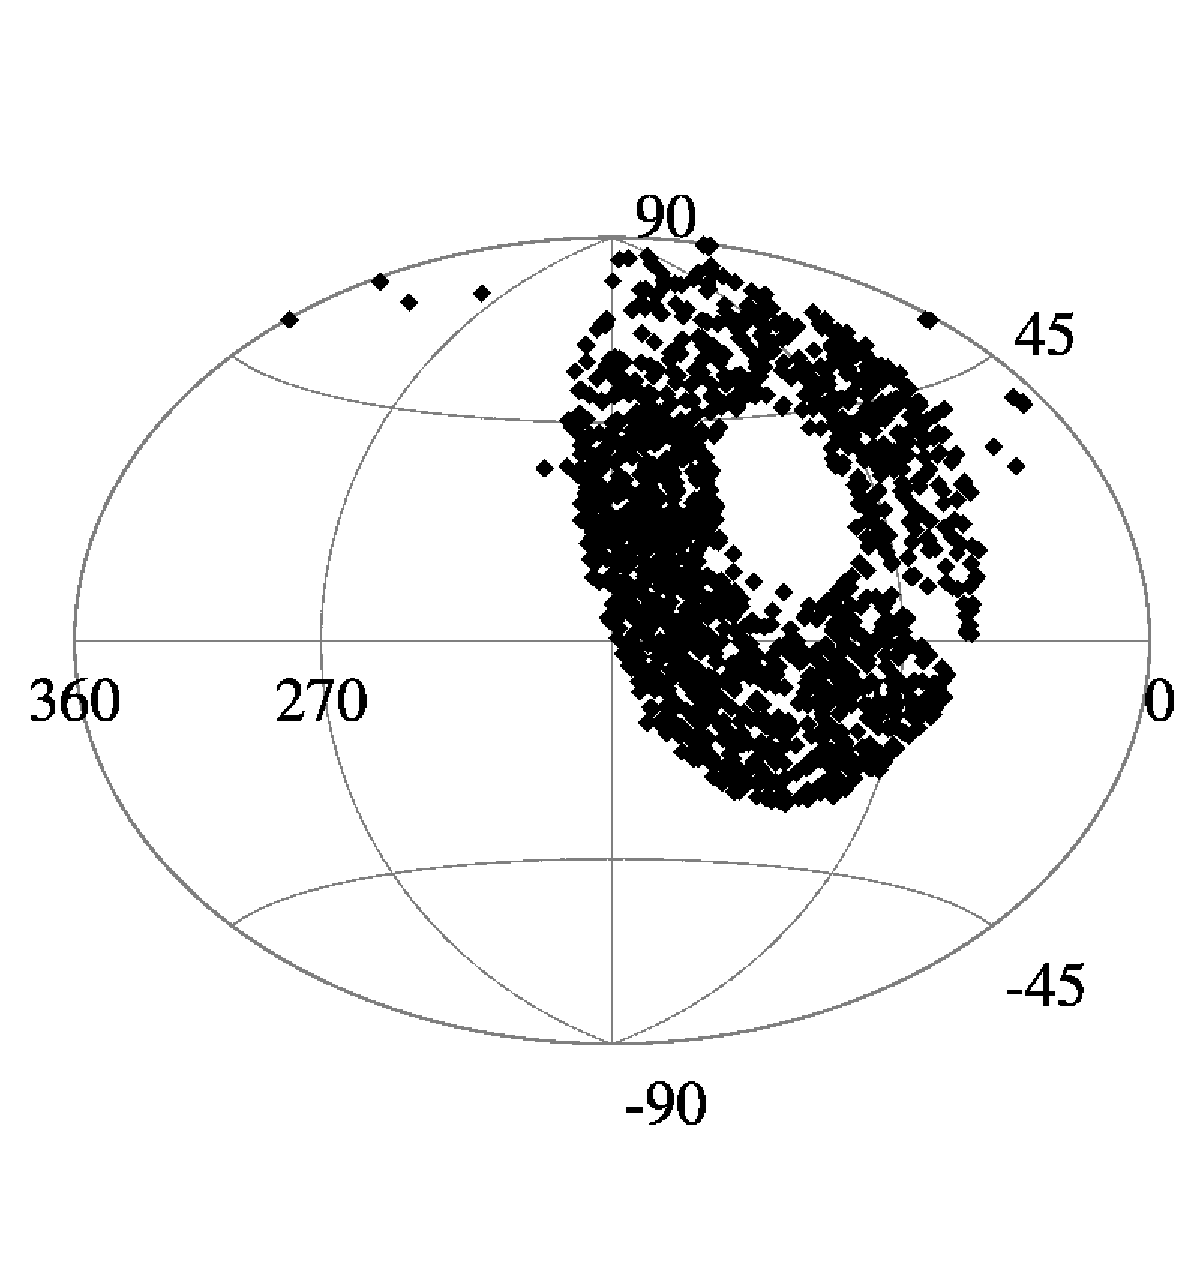
\includegraphics[width=0.49\columnwidth]{fig1_b.eps}
\caption{Распределение звезд пулковской программы по небесной сфере в экваториальной (слева) и галактической (справа) системах координат. Взято из работы~\cite{2015AstL...41..833K}, рис.~1.}
 \label{fig:15alloc}
\end{figure}

Третья часть главы разделена на 3 пункта и посвящена выявлению $\Delta\mu$-двойных звезд. Первый пункт посвящен вычислению порогового значения параметра F. Для этого было проведено численное моделирование движения одиночных звезд с заданными ошибками координат и, соответственно, были вычислены значения вероятности вычисления параметра $F$ для таких объектов. В для разного числа доступных положений получились разные  пороговые значения $F$. Например, в случае 6 точек к кандидатам в $\Delta\mu$-двойные предложено относить звезды, для которых $F>5.3$, в случае 10 точек "--- $F>3.1$. Во втором пункте приведена общая характеристика полученных собственных движений и приведены результаты вычисления параметра $F$. В итоге были обработаны кадры и сканы 1308 объектов, результаты опубликованы в базе CDS\footnote{\textit{http://vizier.u-strasbg.fr/viz-bin/VizieR?-source=J/PAZh/41/896}}. Полученные квазисредние собственные движения характеризуются средней точностью около 5~--~10~$mas/yr$, квази мгновенные "--- 10~--~20~$mas/yr$ (в данном случае величина ошибки сильно зависит от наличия кадров SDSS и блеска звезды). Все результаты были разделены на 2 группы по значению разностей эпох полученных квазимгновенных собственных движений. В первую группу вошли звезды, разность эпох квазимгновенных собственных движений которых составила более 5 лет. Такие собственные движения характеризовались наиболее высокой точностью (в среднем "--- чуть более 4~$mas/yr$). Среди 1065 звезд из первой группы 121 проявила как кандидат в $\Delta\mu$-двойные. Во второй группе оказались звезды, для которых разность эпох квазимгновенных собственных движений не превышала 5 лет. Точность таких собственных движений не превышает 10~$mas/yr$, и среди 243 таких звезд признаки двойственности обнаружили 14 звезд. Однако, результаты второй группы представляются не достаточно надежными, так что дальнейшие исследования в основном проводились для кандидатов, выявленных из первой группы. 

Третий пункт посвящен первичной верификации результатов детектирования $\Delta\mu$-двойных. Примерно 9\,\% из выявленных кандидатов (10 звезд из 121) входят в каталог WDS (в основном это широкие пары), однако среди <<одиночных>> звезд в WDS присутствует примерно 6\,\% (58 из 944), поэтому присутствие в каталоге визуальных двойных звезд является довольно слабым подтверждением эффективности метода. Также 33 программные звезды оказались в параллактической пулковской программе, в ходе которых рассчитывались собственные движения с разностью эпох примерно 3~--~5~лет. На их основе были рассчитаны параметры $F_\pi$ (пороговое значение было оценено как $F_\pi>3$), и было выявлено 18 кандидатов в $\Delta\mu$-двойные (5 присутствуют в каталоге WDS). О корреляции $F_\pi$ со значением $F$ можно говорить с натяжкой. Присутствие в WDS как кандидатов в $\Delta\mu$-двойные, так и <<одиночных>> звезд можно объяснить большими периодами (сотни и тысячи лет) обращения широких пар, которых объяснимое большинство в каталоге визуально-двойных звезд и которые ожидаемо плохо детектируются анализом собственных движений. Также в качестве верификации через shapelet-разложение была оценена асимметрия изображений полученных $\Delta\mu$-двойных. Для оценки эффективности такой верификации была сделана симуляция, в ходе которой оказалось, что оценка асимметрии наиболее эффективна для угловых расстояний 2~--~4~$''$. Учитывая качество изображений и масштабы используемых кадров, было заключенно, что оценка асимметрии может являться в данном контексте только дополнительным фактором наряду с параметром $F$, в финальную таблицу были включены максимальные значения асимметрий по всем обзорам. Среднее значение асимметрии по всем $\Delta\mu$-двойным оказалось 0.039, для <<одиночных>> "--- 0.025. В электронные результаты включены известные значения параметров двойных звезд, приведенных в каталоге WDS. Также вероятным признаком двойственности может служить смещения оптического центра звезды при наблюдениях в оптическом и инфракрасном диапазонах. Эффект такого смещения особенно должен проявляться в звездных парах с коричневыми карликами. Значения таких смещений также включены в таблицу для звезд, присутствующих а обзоре 2MASS. И последним способом верификации, расмотренным в данном разделе, является анализ фотометрических данных. Для этого с применением падуанских изохрон\footnote{\textit{http://stev.oapd.inaf.it/cgi-bin/cmd}} (\cite{2012MNRAS.427..127B},~\cite{2014MNRAS.444.2525C},~\cite{2014MNRAS.445.4287T}) и безансонской модели Галактики~\cite{2003A&A...409..523R} были построеные двуцветные диаграммы для звезд масс от 0.1 до 0.7~$M_{\odot}$, на которые мы нанесли наши $\Delta\mu$-двойные. В результате можно сделать вывод, что такой фотометрический анализ может быть эффектичен для выявления пар <<М-карлик~+~белый карлик>>. Для отдельных объектов каждый из методов верификации показал хорошее соответствие с астрометрическими исследованиями, что позволило нам говорить о потенциале исследования кандидатов и о необходимости адресной проверки кандидатов методами наблюдений высокого разрешения.

В \underline{\textbf{четвертой главе}} дано описание поиска двойных и кратных объектов через анализ их изображений, которому посвящена работа~\cite{2018AstL...44..103K}. Для этого исследования были выбраны звезды, отмеченные флагом <<duplicate source>> в Gaia (относительно таких объектов авторы проекта отмечают возможную проблему кросс-идентификации и необходимость перепроверки данных <<на Земле>>).

Через квадрупольные моменты shaplete-разложения, упомянутые в главе 2, приведены формулы вычисления значений асимметрии и эллиптичности изображения. Описаны этапы выявления двойных систем через анализ изображений:
\begin{enumerate} 
  \item Построение PSF изображения звезы; 
  \item Вычисление оценок асимметрии и эллиптичности;
  \item Верификация через моделирование двойной звезды.
\end{enumerate}
В результате из 702 исследованных данным методом звезд 144 звезды имели значительные значения эллиптичности и/или асимметрии. Из них 6 присутствуют в каталоге WDS.

\underline{\textbf{Пятая глава}} посвящена адресной верификации $\Delta\mu$-двойных звезд черех спекл-интерферометрические наблюдения, которые проводились на двух инструментах: 6--метровом БТА САО РАН и 2,5--метровом КГО ГАИШ МГУ. В первой же сессии наблюдений был получен значимый результат "--- подтверждена двойственность впервые открытой двойной звезды J1158+4239, о чем было изложено в работе~\cite{2016AstL...42..686K}. Для данной системы средневзвешенные параметры на эпоху B2015.88248 таковы: $\rho = 286.2\pm0.9$~mas и $\theta=230.24\pm0.16^\circ$, разность блеска компонент $\Delta m = 0.55\pm0.03$ (фильтр 800/100~нм). Ведутся дополнительные наблюдения для построения орбиты.

Помимо J1158+4239 также подтвеждена двойственность ещё четырех звезд. Дальнейшие исследования продолжаются.

В \underline{\textbf{шестой главе}} представлено сравнение пулковских собственных движений и собственных движений, рассчитанных в проекте Gaia. В Gaia DR2 представлены 684 звезды пулковской программы. Средние разности собственных движений составляют $-0.3\pm5.8$~mas/yr по прямому восхождению и $0.3\pm5.6$~mas/yr по склонению. Из исследованных $\Delta\mu$-двойных 62 звезды присутствуют в Gaia.  Из них 30 имеют значения параметра $F>2.49$. Такой результат с одной стороны может говорить о недостатке нашего исследования (некоторые большие значения F могут быть следствием значительных ошибок, являющихся следствием малого числа точек для вычисления квазимгновенных движений), но с другой стороны большой процент звезд подтвердили свою двойственность. В будущем необходимо провести более скрупулезную работу с привличением собственных движений Gaia, а также точнее изучить пограничное значение критерия $F$. 
%\newpage

В \underline{\textbf{заключении}} приведены основные результаты работы, которые заключаются в следующем:
%% Согласно ГОСТ Р 7.0.11-2011:
%% 5.3.3 В заключении диссертации излагают итоги выполненного исследования, рекомендации, перспективы дальнейшей разработки темы.
%% 9.2.3 В заключении автореферата диссертации излагают итоги данного исследования, рекомендации и перспективы дальнейшей разработки темы.
\begin{enumerate}
 \item Для выполнения поставленных задач были проведены наблюдения на Нормальном астрографе и телескопе <<Сатурн>>;
 \item Для обработки полученных наблюдений был исследован и адаптирован метод shapelet-разложения;
   \item Для получения прочих материалов исследования, численных расчетов и построения промежуточных моделей было создано специализированное программное обеспечения на C++ и Python;
 \item На основе анализа собственных движений 1308 быстрых звезд было выявлен 121 кандидат в $\Delta\mu$-двойные, по данному исследованию опубликована работа \cite{2015AstL...41..833K};
 \item Были проведены дополнительные спекл-интерферометрические исследования 7 программных звез, для пяти из которых были подтверждены статусы двойных (присутствие 2х из них в каталоге WDS может служить фактором верификации исследования), по выявлению одной из звезд опубликована работа \cite{2016AstL...42..686K} и уже получены наблюдения, позволяющие построить её предварительную орбиту;
   \item В результате анализа форм изображений 702 звезд (отмеченных в Gaia DR2 флагом \glqq duplicate source\grqq ) было выявлено ещё 138 кандидатов в двойные, по данному исследованию также написана статья \cite{2018AstL...44..103K}.
\end{enumerate}


%При использовании пакета \verb!biblatex! список публикаций автора по теме
%диссертации формируется в разделе <<\publications>>\ файла
%\verb!common/characteristic.tex!  при помощи команды \verb!\nocite!

\ifdefmacro{\microtypesetup}{\microtypesetup{protrusion=false}}{} % не рекомендуется применять пакет микротипографики к автоматически генерируемому списку литературы
\ifnumequal{\value{bibliosel}}{0}{% Встроенная реализация с загрузкой файла через движок bibtex8
  \renewcommand{\bibname}{\large \bibtitleauthor}
  \nocite{*}
  \insertbiblioauthor           % Подключаем Bib-базы
  %\insertbiblioexternal   % !!! bibtex не умеет работать с несколькими библиографиями !!!
}{% Реализация пакетом biblatex через движок biber
  \ifnumgreater{\value{usefootcite}}{0}{
%  \nocite{*} % Невидимая цитата всех работ, позволит вывести все работы автора
  \insertbiblioauthorcited      % Вывод процитированных в автореферате работ автора
  }{
  \insertbiblioauthor           % Вывод всех работ автора
%  \insertbiblioauthorgrouped    % Вывод всех работ автора, сгруппированных по источникам
%  \insertbiblioauthorimportant  % Вывод наиболее значимых работ автора (определяется в файле characteristic во второй section)
  \insertbiblioexternal            % Вывод списка литературы, на которую ссылались в тексте автореферата
  }
}
\ifdefmacro{\microtypesetup}{\microtypesetup{protrusion=true}}{}

%\newpage
\section*{Работы, опубликованные по теме диссертации}

\begin{enumerate}
 \item M. Y. Khovritchev, A. M. Kulikova <<$\Delta\mu$–binaries among stars with large proper motions>> Astronomy Letters. –– 2015. –– Dec. –– Vol. 41, no. 12. –– P. 833––847.;
 \item M. Y. Khovrichev et al. <<Detection of the binarity of the star J1158+4239>> Astronomy Letters. –– 2016. –– Oct. –– Vol. 42, no. 10. –– P. 686––692.;
 \item M. Y. Khovrichev et al. <<Searching for Binary Systems Among Nearby Dwarfs Based on Pulkovo Observations and SDSS Data>> Astronomy Letters. ––
2018. –– Feb. –– Vol. 44, no. 2. –– P. 103––118..
\end{enumerate}
      % Содержание автореферата

%%% Выходные сведения типографии
\newpage\thispagestyle{empty}

\vspace*{0pt plus1fill}

\small
\begin{center}
    \textit{\thesisAuthor}
    \par\medskip
    
    \thesisTitle
    \par\medskip
    
    Автореф. дис. на соискание ученой степени \thesisDegreeShort
    \par\bigskip
    
    Подписано в печать \blank[\widthof{999}].\blank[\widthof{999}].\blank[\widthof{99999}].
    Заказ № \blank[\widthof{999999999999}]
    
    Формат 60\(\times\)90/16. Усл. печ. л. 1. Тираж 100 экз.
    %Это не совсем формат А5, но наиболее близкий, подробнее: http://ru.wikipedia.org/w/index.php?oldid=78976454
    
    Типография \blank[0.5\linewidth]
\end{center}
\cleardoublepage

\end{document}
